\documentclass{article}

\usepackage[tmargin=.9in, bmargin=.9in, lmargin=1in, rmargin=1in]{geometry}
\usepackage{bookmark, wrapfig, enumitem, pdflscape, hyphenat}
\usepackage[labelfont=bf]{caption}
\usepackage{lmodern}
\usepackage[sfdefault]{roboto}
\usepackage[T1]{fontenc}

\usepackage{graphicx}
    \makeatletter % tex.stackexchange.com/a/28565
    \setlength{\@fptop}{0pt}
    \setlength{\@fpbot}{0pt plus 1fil}
    \makeatother

\usepackage[absolute, overlay]{textpos}
    \setlength{\TPHorizModule}{1mm}
    \setlength{\TPVertModule}{1mm}

\usepackage{xcolor}
    \definecolor{WCM}{RGB}{172,31,44} % AC1E2C

\usepackage{hyperref} \hypersetup{
    colorlinks=true, linkcolor={blue!65!black},
    citecolor={blue!65!black}, urlcolor={blue!50!black},
    pdfpagelayout=OneColumn, pdfstartview={XYZ null null 1.25},
    bookmarksnumbered=true, bookmarksopen=true, bookmarksopenlevel=3
}

\usepackage[backend=bibtex, style=nature]{biblatex}
    \addbibresource{latex/references.bib}

\newcommand{\beginsupplement}{
% bytesizebio.net/2013/03/11/adding-supplementary-tables-and-figures-in-latex
    \newpage
    \setcounter{page}{1}
    \renewcommand{\thepage}{S-\arabic{page}}
    \setcounter{table}{0}
    \renewcommand{\thetable}{S\arabic{table}}
    \setcounter{figure}{0}
    \renewcommand{\thefigure}{S\arabic{figure}}
 }

\usepackage{setspace}

\begin{document}

\begin{center}
    \Large{\textbf{Haplotype Diversity and Sequence Heterogeneity of Human Telomeres}}
    \\~\\
    \small{
        Kirill Grigorev\textsuperscript{1,2 \#},
        Jonathan Foox\textsuperscript{1,2,3 \#},
        Daniela Bezdan\textsuperscript{1,2,3},
        Daniel Butler\textsuperscript{1},
        Jared J. Luxton\textsuperscript{4,5},
        Jake Reed\textsuperscript{1},
        \\%rem
        Miles J. McKenna\textsuperscript{4,5},
        Lynn Taylor\textsuperscript{4,5},
        Kerry A. George\textsuperscript{4,5},
        Cem Meydan\textsuperscript{1,2,3},
        Susan M. Bailey\textsuperscript{4,5 *},
        Christopher E. Mason\textsuperscript{1,2,3,6 *}
    }
\end{center}

\small{ \noindent
    \textsuperscript{1} Department of Physiology and Biophysics, Weill Cornell Medicine, New York, New York, USA
    \\
    \textsuperscript{2} The HRH Prince Alwaleed Bin Talal Bin Abdulaziz Alsaud Institute for Computational Biomedicine, \\
    \textcolor{white}{\textsuperscript{2}} Weill Cornell Medicine, New York, New York, USA
    \\
    \textsuperscript{3} The Feil Family Brain and Mind Research Institute, New York, New York, USA
    \\
    \textsuperscript{4} Department of Environmental and Radiological Health Sciences, Colorado State University, Fort Collins, CO
    \\
    \textsuperscript{5} Cell and Molecular Biology Program, Colorado State University, Fort Collins, CO
    \\
    \textsuperscript{6} The WorldQuant Initiative for Quantitative Prediction, Weill Cornell Medicine, New York, NY, USA
    \\
    \textsuperscript{\#} Co-first authors
    \\
    \textsuperscript{*} Corresponding authors. Send correspondence to S.M.B. (susan.bailey@colostate.edu) \\%rem
    \textcolor{white}{\textsuperscript{*}} and C.E.M. (chm2042@med.cornell.edu)
}

\normalsize
\doublespacing

\section*{Abstract} \addcontentsline{toc}{section}{Abstract}
Telomeres are regions of repetitive nucleotide sequences capping the ends of eukaryotic chromosomes that protect against deterioration, and whose lengths can be correlated with age and adverse health risk factors.
Given their length and repetitive nature, telomeric regions are not easily reconstructed from short-read sequencing, making telomere sequence resolution a very costly and generally intractable problem.
Recently, long-read sequencing, with read lengths measuring in hundreds of Kbp, has made it possible to routinely read into telomeric regions and inspect their sequence structure.
Here, we describe a framework for extracting telomeric reads from single-molecule sequencing experiments, describing their sequence variation and motifs, and for haplotype inference.
We find that
long telomeric stretches can be accurately captured with long-read sequencing,
observe extensive sequence heterogeneity of human telomeres,
discover and localize non-canonical motifs (both previously reported as well as novel),
confirm the presence of the non-canonical motifs in short read sequencing experiments,
and report the first motif composition maps of human telomeric diplotypes on a multi-Kbp scale.
%TODO stress scalability, approachability of PacBio WGS for this purpose
%TODO stress that it is de novo and capable of finding previously known AND novel motifs
%TODO haplotype spectra, not diplotypes

\section*{Keywords} \addcontentsline{toc}{section}{Keywords}
Telomere, telomeric haplotypes, long-read sequencing, telomere sequence heterogeneity

\pagebreak
%\singlespacing
%\tableofcontents
\doublespacing

\section*{Introduction} \addcontentsline{toc}{section}{Introduction}
Telomeres are the functional ends of human chromosomes that naturally shorten with cell division and therefore with age \cite{teloaging}.
Telomere length can also be influenced by a variety of lifestyle factors and environmental exposures (e.g., stress, exercise, air pollution, radiation) \cite{teloeffects}.
While human telomeres are known to consist largely of a conserved six-nucleotide repeat (TTAGGG) \cite{moyzis}, several studies have identified variations of this motif in proximal telomeric regions \cite{telovars1989,telovars1999,telovars2018,telovars2019}.
However, such studies were performed with oligonucleotide hybridization, PCR, immunoprecipitation, and short-read sequencing, resulting in discovery, but not localization, of motif variants. %TODO not quite true, but old research still fundamentally lacking - reword!
Thus, long-range maps of telomeric sequence variation in the human genome are still lacking.
Such maps can provide insight into telomere biology and enable novel approaches to analyze the effects of health status, aging, and environment on telomere structure and length. %TODO better wording and points
\\~\\
To improve our understanding of telomere sequence structure and variation, we developed \textit{edgeCase}, a framework for alignment, motif discovery, and haplotype inference from human telomeric reads. %TODO haplotyle spectra!
We have validated these methods using Genome in a Bottle \cite{giab} single-molecule real-time (SMRT) sequencing datasets generated with Pacific Biosciences circular consensus sequencing (PacBio CCS) \cite{pacbio,pacbioccs}, and short-read Illumina \cite{illumina} and 10X Genomics (Chromium) \cite{10x} datasets.
These results provide evidence for multiple novel, non-canonical telomeric repeats, resolution of chromosome-specific diplotypes with SMRT sequencing, and a new method for long-range characterization of the structure of telomeric sequences. %TODO not diplotypes, better!

\section*{Results} \addcontentsline{toc}{section}{Results}

\subsection*{Telomeric reads are present in human long-read whole genome sequencing datasets} %TODO highlight hg38ext in subsection title
\addcontentsline{toc}{subsection}{Telomeric reads are present in human long-read whole genome sequencing datasets} %TODO mention protocol / ext
We aligned PacBio CCS reads of three Genome in a Bottle (GIAB) human subjects (HG001, HG002, and HG005) to a combination of the human reference genome and human subtelomeric assemblies (see \hyperref[sec:methods]{Materials and Methods}). %TODO describe how to obtain
In total, we observed reads mapping to the ends of chromosomes and extending into telomeric regions on 9 \textit{p} arms and 17 \textit{q} arms, with 256 such reads ($\sim$10x mean coverage) in the HG001 dataset, 570 ($\sim$22x) in HG002, and 241 ($\sim$9x) in HG005.
\autoref{fig:hg002_alignment} schematically represents the alignment of such reads in the HG002 dataset; alignment plots for the other two datasets are available as a supplemental figure (\autoref{fig:hg00x_alignments}), and full mapping statistics are available \mbox{in \autoref{tab:telomeric_read_counts}}. %TODO reword to describe protocol, Figure illustrates protocol, Table provides mapping stats
%TODO move support a few sections forward
Illumina reads from matching GIAB datasets supported 70.8\%, 63.3\%, and 82.7\% of the candidate PacBio CCS sequence, %TODO w/o direct support
providing average coverages of $\sim$5x, $\sim$9x, and $\sim$6x, respectively. %TODO new numbers; TODO recalculate coverage or refer to Table

\subsection*{Telomeric reads contain variations of the canonical motif}
\addcontentsline{toc}{subsection}{Telomeric reads contain variations of the canonical motif}
We performed \textit{de novo} repeat discovery %FIXME in the supported regions
for motifs of lengths 4 through 16 and identified motifs in repeat contexts that are statistically enriched in the three datasets.
The majority of motifs were either the canonical TTAGGG / CCCTAA, its variations (e.g., TT\underline{G}GGG / CCC\underline{C}AA), or a duplet of variants, such as TTAGGGTTA\underline{G}GGG (\autoref{tab:repeatfinder_full}).
CG-rich motifs were also observed on the \textit{p} arms.
The top enriched motif (TTAGGG / CCCTAA) explained 43.3\%\textendash{}54.4\% of the telomeric repeat content on the \textit{q} arms, and 10.0\%\textendash{}22.7\% on the \textit{p} arms, %TODO use recalculated values
%FIXME while overall, four motifs on the \textit{q} arms and three motifs on the \textit{p} arms each explained at least 0.5\% of the repeat content.
These top motifs, as well as 15 less enriched ones, were confirmed in independently generated human short read and linked-read genomic datasets (\hyperref[sec:supp_methods]{Supplemental methods}, \autoref{tab:shortread_repeatfinder}). %TODO See MAIN methods now
%TODO "N" (top?) enriched motifs
%TODO mention that they confirm only the existence of motifs, but not the locations, because they cannot.
% ?? out of ?? (??.?\%) of these motifs were confirmed in independently generated human linked-read, short read genomic, and short read transcriptomic datasets (\hyperref[sec:supp_methods]{Supplemental methods}, \autoref{tab:shortread_repeatfinder}).
\autoref{fig:hg002_densityplot_q_arm} visualizes the locations of the top four enriched motifs on the \textit{q} arm of the HG002 dataset; only the arms covered by at least 25 reads are displayed. %TODO p+q
Plots for other datasets and arms are available as supplemental figures: \autoref{fig:hg002_densityplot_p_arm} visualizes the top three motifs on the \textit{p} arm of the HG002 dataset, \autoref{fig:hg001_densityplots} and \autoref{fig:hg005_densityplots} visualize datasets HG001 and HG005 respectively. %TODO: all other datasets in Supplement
Long reads on each arm agreed on the locations of different motifs within any given 10 bp window (the median of normalized Shannon entropy was 0.000 for all data, and the 3rd quartile was 0.166, 0.074, and 0.211 for the three datasets, respectively, \autoref{fig:entropy}), indicating that locations of the variations are colinear among reads and are not a result of sequencing errors. %TODO new 3rd quartile values
%FIXME move "not a result of sequencing errors to next section, expand on potential causes of third quartile

\subsection*{Long-read sequencing resolves human telomeric haplotypes} %TODO rename to something about "variation," "spectra," etc.
\addcontentsline{toc}{subsection}{Long-read sequencing resolves human telomeric haplotypes}
%TODO discuss causes of entropy: seq. errors, SV, haplotypes
%TODO rewrite this entire section!
Sequences of telomeric reads clustered by relative pairwise Levenshtein distances \cite{levenshtein} with varying levels of heterogeneity depending on the dataset and the chromosomal arm to which they belonged.
We examined the \textit{q} arms of the HG002 dataset to investigate this heterogeneity, as they provided the deepest coverage (\autoref{tab:telomeric_read_counts}), and found that, on 12 out of the 15 arms, reads clustered into two prominent groups per arm when maximizing the Bayesian information criterion \cite{bic} (see \hyperref[sec:methods]{Materials and Methods}).
Pairwise distances between the reads within these clusters were significantly lower than those for out-of-cluster pairings, implying that distinct telomeric haplotypes are present.
To quantify the differences between putative haplotypes, we calculated silhouette scores \cite{silhouette} for these clusterings (\autoref{tab:levenshtein-q_arm}), and generated motif density plots for the four chromosome arms with the highest such scores to visualize the differences in haplotypes (\autoref{fig:levenshtein_q_arm}).

\section*{Discussion} \addcontentsline{toc}{section}{Discussion}
Repeat-rich, low-complexity regions of the human genome such as telomeres have been historically recalcitrant to full mapping and annotation \cite{miga2015}, mainly due to the alignment challenge they pose and to the read lengths required to span such areas \cite{ngslowcomplexity}.
The advent of long-read, single-molecule methods (third generation sequencing) has provided new opportunities to map the sequence composition of a previously "dark" area of the human genome, enabling research into the sequence composition and length dynamics \cite{luxton2020} of telomeres. %TODO add Luxton ref.
Our results reaffirm that the canonical repeat (TTAGGG) is certainly the most dominant type of motif in telomeres, but also reveal a surprising diversity of repeat variations, which are confirmed by both short and long-read sequencing technologies.
This diversity of repeats includes previously reported variants, as well as novel motifs that are characterized not only by nucleotide substitutions, but also insertions, deletions, and even motif pairing.
Apart from these variations, CG-rich motifs were identified in telomeric regions of \textit{p} arms, consistent with previously reported findings \cite{cpg}.
Moreover, while short read sequencing is able to identify such variants, it alone cannot reveal the relative locations of these motifs within telomeres, as repetitive short reads can neither be aligned outside of the reference genome nor provide enough overlap variability to be assembled \textit{de novo}. %TODO stress that it is de novo and novel; TODO contrast with old methods, not only with SR seq XXX!!!
Long SMRT reads, on the other hand, can be anchored to known subtelomeric sequences of the human genome and extend into the previously unmapped telomeric area.
These results also highlight the need of better subtelomeric and telomeric annotations in the human genome.
Four of the 40 subtelomeric assemblies \cite{riethman2014} were homologous to regions in the reference genome far within the respective chromosomes (up to 586 Kbp into the reference sequence), and the canonical motif was present on the \textit{q} arm of chr8 only after 2\textendash{}3Kbp past the annotated boundary in all datasets, suggesting that the existing assemblies do not provide a completely accurate telomeric annotation, and that methods described herein could help to resolve these areas of reference genomes.
\\~\\
We observed PacBio CCS reads reaching up to 16 Kbp beyond the known regions of the genome, and resolving the underlying sequence with reasonable fidelity, measured both by the entropy of motif assignment and by pairwise Levenshtein distances between the reads belonging to the same chromosomal arms.
While short reads also provided support for non-canonical motifs, the overlap between the short and the long reads was substantial, but not complete, which can be explained by the necessary bias towards the canonical motif during the selection of short reads.
Therefore, telomeric regions with higher content of non-canonical repeats are less likely to be identified through the use of short reads, and instead, long reads appear to be more suitable for this purpose as well. %TODO as well as for the purpose of long-range mapping XXX!!
The identified variations in long range contexts enable clustering of SMRT reads into distinct haplotypes at ends of chromosomes, and thus provide a new means of diplotype mapping and reveal the existence and motif composition of such diplotypes on a multi-Kbp scale.
%TODO paragraph about re-clustered spectra constrained to subjects, suggest multiple haplotypes, talk about cell types, the need to sequence deeper and maybe cell-specific seq.
%XXX for reviewers: stress that the shift from diplotypes to spectra does not invalidate the previous findings: we were able to put these findings and the method into a broader context and see more structure.

\section*{Materials and Methods} \addcontentsline{toc}{section}{Materials and Methods} \label{sec:methods}

\subsection*{The extended reference genome}
\addcontentsline{toc}{subsection}{The extended reference genome}
We constructed the extended reference genome by performing an all-to-all alignment of all contigs in the \textit{hg38} reference genome \cite{grch38,hg38} and the subtelomeric assemblies \cite{riethman2014} with \textit{minimap2} \cite{minimap} using three settings for assembly-to-reference mapping (\textit{asm5}, \textit{asm10}, \textit{asm20}).
Forty subtelomeric contigs mapped to ends of \textit{hg38} chromosomes with a mapping quality of 60, one (XpYptel) mapped with the quality of 0 and was discarded; one (14qtel) mapped to the ALT version of chr14 (chr14\_KI270846v1\_alt) with the quality of 52, which, in turn, mapped to the main chr14 chromosome with the quality of 60. %TODO stress that the mappings were perfect (CIGAR)
%Finally, an ALT version of chr12 (chr12\_GL877875v1\_alt) mapped to chr12 and an unplaced chrUn\_KI270745v1 to chr17, both with the quality of 60.
These data and the exact match and mismatch coordinates were used to create a combined reference (\textit{hg38ext}) in which subtelomeric contigs informed the locations of the boundaries of the telomeric tracts (\textit{tract\_anchor}).
Such contigs that mapped fully within \textit{hg38} chromosomes resulted in \textit{tract\_anchor} annotations directly on those \textit{hg38} chromosomes; partially mapping contigs were considered as forking from the \textit{hg38} sequence and were similarly annotated by themselves.

\subsection*{Detection of telomeric sequences in long-read datasets}
\addcontentsline{toc}{subsection}{Detection of telomeric sequences in long-read datasets}
Three subjects were selected for the analysis. %TODO obviously, seven now
The first individual (NA12878/HG001) came from the pilot genome of the HapMap project \cite{HG001}, while the other two, including the son from the Ashkenazi Jewish Trio (NA24385/HG002) and the son from the Chinese Trio (NA24631/HG005), are members of the Personal Genome Project, whose genomes are consented for commercial redistribution and reidentification \cite{HG00X}. %TODO provenance of all
These subjects are referred to hereafter as HG001, HG002, and HG005, respectively. %TODO all seven
\\~\\
For subjects HG001 and HG005, Genome in a Bottle \cite{giab} PacBio\_SequelII\_CCS\_11kb datasets were used (one dataset per each subject).
For subject HG002, a combination of two sequencing experiments was analyzed (PacBio\_CCS\_10kb and PacBio\_CCS\_15kb). %TODO list all datasets
The mean coverage was $\sim$29x, $\sim$58x, and $\sim$32x for subjects HG001, HG002, and HG005, respectively. %TODO recalc new coverages
Reads were mapped to \textit{hg38ext} with \textit{minimap2}, and reads that mapped to either end of either chromosome and overlapped the boundary of its telomeric tract were selected for further analysis. %TODO re-reference Figure 1
These reads had a portion of their sequence mapped to the reference contig and a portion extending beyond the reference (soft- or hard-clipped in the alignment file).
Sequences past the \textit{tract\_anchor} marker were extracted from the reads that had this marker within their mapped portion (from the 5' end to the marker on \textit{p} arms and from the marker to the 3' end on \textit{q} arms, accounting for forward and reverse mappings).
%TODO move the short-read paragraph into a later Validation section, together with real humans
To identify regions of the telomeres that are fully supported by both short and long reads, we extracted candidate telomeric reads from GIAB Illumina datasets
   (NIST\_NA12878\_HG001\_HiSeq\_300x,
    NIST\_HiSeq\_HG002\_Homogeneity-10953946,
    HG005\_NA24631\_son\_HiSeq\_300x;
    all three $\sim$300x coverage)
with \textit{Telomerecat} \cite{telomerecat}, and selected those that mapped perfectly with \textit{minimap2} (at least a 50bp-long exact match without insertions or deletions, allowing all secondary mappings) to the telomeric regions of the PacBio CCS candidates from the same subject's dataset. %TODO describe new approach and reference supplemental figure

\subsection*{Detection of telomeric sequences in short- and linked-read datasets} %TODO "Validation," include GIAB short reads here XXX!!
\addcontentsline{toc}{subsection}{Detection of telomeric sequences in short- and linked-read datasets}
To evaluate sequence motifs in datasets generated by technologies other than SMRT, we generated four whole-genome Illumina datasets (mean coverage $\sim$104x) and three linked-read 10X datasets (mean coverage $\sim$28x) for one individual at different timepoints aboard the International Space Station (ISS), and one additional linked-read 10X dataset (coverage $\sim$47x) for another individual aboard the ISS.
%TODO stress non-cell lines, real humans; argument about non-LONG-READS as a separate phrase.
Blood samples were collected from astronaut subjects as described in \cite{twins_study}. %TODO cite Garrett-Bakelman 2019
For each sample, 1.2ng of sorted immune cell input was aliquoted for TruSeq PCR-free WGS (short read) and standard Chromium 10X whole genome (linked-read) preparation respectively, and sequenced across one S4 flow cell on an Illumina NovaSeq 6000.
From these datasets, candidate telomeric short reads were selected using Telomerecat \cite{telomerecat}.

\subsection*{Identification of repeat content}
\addcontentsline{toc}{subsection}{Identification of repeat content}
Overrepresentation of motifs of lengths $k \subset [4 .. 16]$ was tested within the candidate telomeric regions of PacBio CCS reads, as well as in the candidate reads from independently generated Illumina and 10X Chromium datasets.  %TODO make sure to define or redefine "telomeric regions"
To target motifs in repeat contexts, doubled sequences (for example, \textit{k}-mer ACGTACGT for motif ACGT) were counted with \textit{jellyfish} \cite{jellyfish}, and counts of \textit{k}-mers synonymous with respect to circular shifts (for example, ACGTACGT and CGTACGTA) were summed together.
For each such \textit{k}-mer, Fisher's exact test was performed to determine whether its count is significant on the background of counts of other \textit{k}-mers of the same length.
Briefly, we considered \textit{k}-mers with counts higher than 1.5 interquartile range above the third quartile of the distribution as potentially classifiable, and a 2\texttimes{}2 contingency matrix $ C $ for the test was constructed as follows:
row 0 contained counts of potentially classifiable \textit{k}-mers,
row 1 contained counts of remaining (non-classifiable) \textit{k}-mers,
columns 0 and 1 contained counts of single and remaining (background) \textit{k}-mers, respectively,
i.e.:
$ C_{0,0} = $ {\rmfamily count of target \textit{k}-mer},
$ C_{0,1} = $ {\rmfamily sum of counts of other potentially classifiable \textit{k}-mers},
$ C_{1,0} = $ {\rmfamily median count of \textit{k}-mer},
$ C_{1,1} = $ {\rmfamily sum of counts of other non-classifiable \textit{k}-mers}.
The resultant \textit{p}-values for each motif among the samples were combined using the Mudholkar-George method \cite{george} within each technology (PacBio CCS, Illumina, 10X Genomics), and the Bonferroni multiple testing correction was applied
Motifs in the long-read datasets for which \textit{k}-mers yielded \textit{p}-values below the cutoff of 0.05 were reported. %TODO Table
Additionally, motifs that were significantly enriched in the datasets produced by all three technologies (PacBio, Illumina, 10X), with respect to reverse-complemented equivalence, were reported. %TODO Supplemental table

\subsection*{Evaluation of sequence concordance in telomeric long reads}
\addcontentsline{toc}{subsection}{Evaluation of sequence concordance in telomeric long reads}
As telomeric reads contain long low-complexity regions and present an alignment challenge, we evaluated concordance of their sequences without realignment of their portions that extended past the reference sequence.
To that end, for all reads mapping to the same chromosomal arm, we calculated densities of each identified motif in a rolling window starting from the innermost mapped position of each entire read.
To evaluate whether the reads on the same arm agree on the positions of different motifs, for each read, we calculated motif densities in 10 bp windows with 10 bp smoothing to buffer insertions and deletions.
For each window in each read, the motif with the highest density was selected to represent that window.
Then, normalized Shannon entropy among all reads was calculated in each window as $ S = \frac{ - \sum_{i} \; ( p_{i} ln p_{i} )}{ln N} $, where $ p_{i} $ is the frequency of each motif in the window and $ N $ is the number of motifs \cite{hepc_entropy}.
The value of normalized entropy was a metric bounded by $ [ 0, 1 ] $, with $ 0 $ describing perfect agreement and $ 1 $ describing maximum randomness.
For visualization, we performed 1000 rounds of bootstrap of the calculated density values in the 10 bp rolling windows, and selected the lower and the upper bounds of the 95\% confidence interval of bootstrap.
Of note, several chromosome arms had the \textit{tract\_anchor} position further away from the end of the contig than others ($\sim$79\textendash{}586 Kbp into the chromosome sequence), and the reads mapping to these arms did not contain these motifs, suggesting that either their subtelomeric annotations were incorrect or large insertions or duplications were present in the reference genome; in light of this, reads mapping to the \mbox{\textit{p} arm} of chr1, the \textit{q} arm of chr4, and both arms of chr20 were removed from the study, and the analysis was repeated.

\subsection*{Extraction of telomeric haplotypes from long-read datasets} %TODO rewrite whole section to talk about spectra XXX!!
\addcontentsline{toc}{subsection}{Extraction of telomeric haplotypes from long-read datasets}
Within groups of reads mapping to each chromosome arm, all relative pairwise Levenshtein distances were calculated. %TODO explain it's edit dist
In short, to calculate the absolute distance between each pair of reads, the sequences in the overlapping positions of the reads were extracted; the distance then equaled the minimum number of single-character insertions, deletions, and substitutions required to make these sequences identical. %TODO explain calculation a bit more
The relative distance was computed as the absolute distance divided by the length of the overlap.
Relative distances were then clustered using Ward's method via the Euclidean metric.
%TODO write so much here XXX XXX XXX XXX!!!
%The optimal number of clusters was determined by maximizing the Bayesian information criterion \cite{bic}, allowing for no more than one outlier and at least five reads per cluster, and silhouette scores for these clusterings were calculated.
%Briefly, as previously described \cite{silhouette}, a silhouette score of a clustering was computed as the mean value of silhouette coefficients of all entries, which, in turn, equaled $ (b - a) \over{max(a, b)} $ where $ a = $ {\rmfamily mean intra-cluster distance} and $ b = $ {\rmfamily mean nearest-cluster distance} for an entry.
%Levenshtein distances of all within-cluster pairings and of all out-of-cluster pairings were compared using the one-tailed Mann-Whitney U test; \textit{p}-values were adjusted with the Bonferroni correction.
%Distinct clusters of reads within the same chromosome arm (adjusted Mann-Whitney U \textit{p}-value below 0.05) were reported as putative haplotypes.
%As the HG002 dataset was combined from two sequencing experiments, we investigated the provenance of reads in these haplotypes; reads from both sequencing experiments contributed to each haplotype with an average $\sim$1:2 ratio (\autoref{tab:hg002_haplotype_assignment}).

\section*{Data access} \addcontentsline{toc}{section}{Data access}
The NASA Life Sciences Data Archive (LSDA) is the repository for all human and animal research data, including the whole genome Illumina and 10X Chromium sequencing datasets from subjects aboard the ISS that were used in this study.
These datasets are protected by the terms of the Weill Cornell Medicine Internal Review Board (IRB) and can be made available to be shared upon request.
LSDA has a public facing portal where data requests can be initiated (\href{https://lsda.jsc.nasa.gov/Request/dataRequestFAQ}{lsda.jsc.nasa.gov/Request/dataRequestFAQ});
the LSDA team provides the appropriate processes, tools, and secure infrastructure for archival of experimental data and dissemination while complying with applicable rules, regulations, policies, and procedures governing the management and archival of sensitive data and information.
The LSDA team enables data and information dissemination to the public or to authorized personnel either by providing public access to information or via an approved request process for information and data from the LSDA in accordance with NASA Human Research Program and JSC Institutional Review Board direction.
\\~\\
%\section*{Availability and implementation} \addcontentsline{toc}{section}{Availability and implementation}
The software for identification of telomeric reads, \textit{de novo} discovery of repeat motifs, haplotype inference and motif density visualization was implemented in Python and is freely available at \\%rem
\href{https://github.com/lankycyril/edgecase}{github.com/lankycyril/edgecase}.

\section*{Acknowledgements} \addcontentsline{toc}{section}{Acknowledgements}
We would like to thank
the Epigenomics Core Facility at Weill Cornell Medicine,
the Scientific Computing Unit (SCU),
XSEDE Supercomputing Resources,
as well as
the STARR grants I9-A9-071, I13-0052,
The Vallee Foundation,
The WorldQuant Foundation,
The Pershing Square Sohn Cancer Research Alliance,
NASA (NNX14AH51G, NNX14AB02G, NNX17AB26G),
The National Institutes of Health (R01MH117406, \\%rem
R01NS076465, R01CA249054, R01AI151059, P01HD067244, P01CA214274),
TRISH (NNX16AO69A:0107, \\%rem
NNX16AO69A:0061),
the LLS (9238-16, Mak, MCL-982, Chen-Kiang),
and
the NSF (1840275).

\section*{Author contributions} \addcontentsline{toc}{section}{Author contributions}
S.M.B. and C.E.M. conceived the study.
K.G., J.F., and C.E.M. developed the framework and analyzed the data.
D.Bu., J.J.L., M.J.M., L.T., and K.A.G. participated in collection and processing of the ISS samples.
D.Be., D.Bu., J.J.L, J.R., and C.M. analyzed the data.
All authors edited the manuscript.

\section*{Competing interests} \addcontentsline{toc}{section}{Competing interests}
The authors declare no relevant conflict of interest, although C.E.M. is a Co-Founder of Onegevity.

\section*{References} \addcontentsline{toc}{section}{References}
\begingroup \raggedright \singlespacing \printbibliography[heading=none] \endgroup

% \pagebreak
% \section*{Figures} \addcontentsline{toc}{section}{Figures}
% 
% \begin{figure}[h!] \centering
% 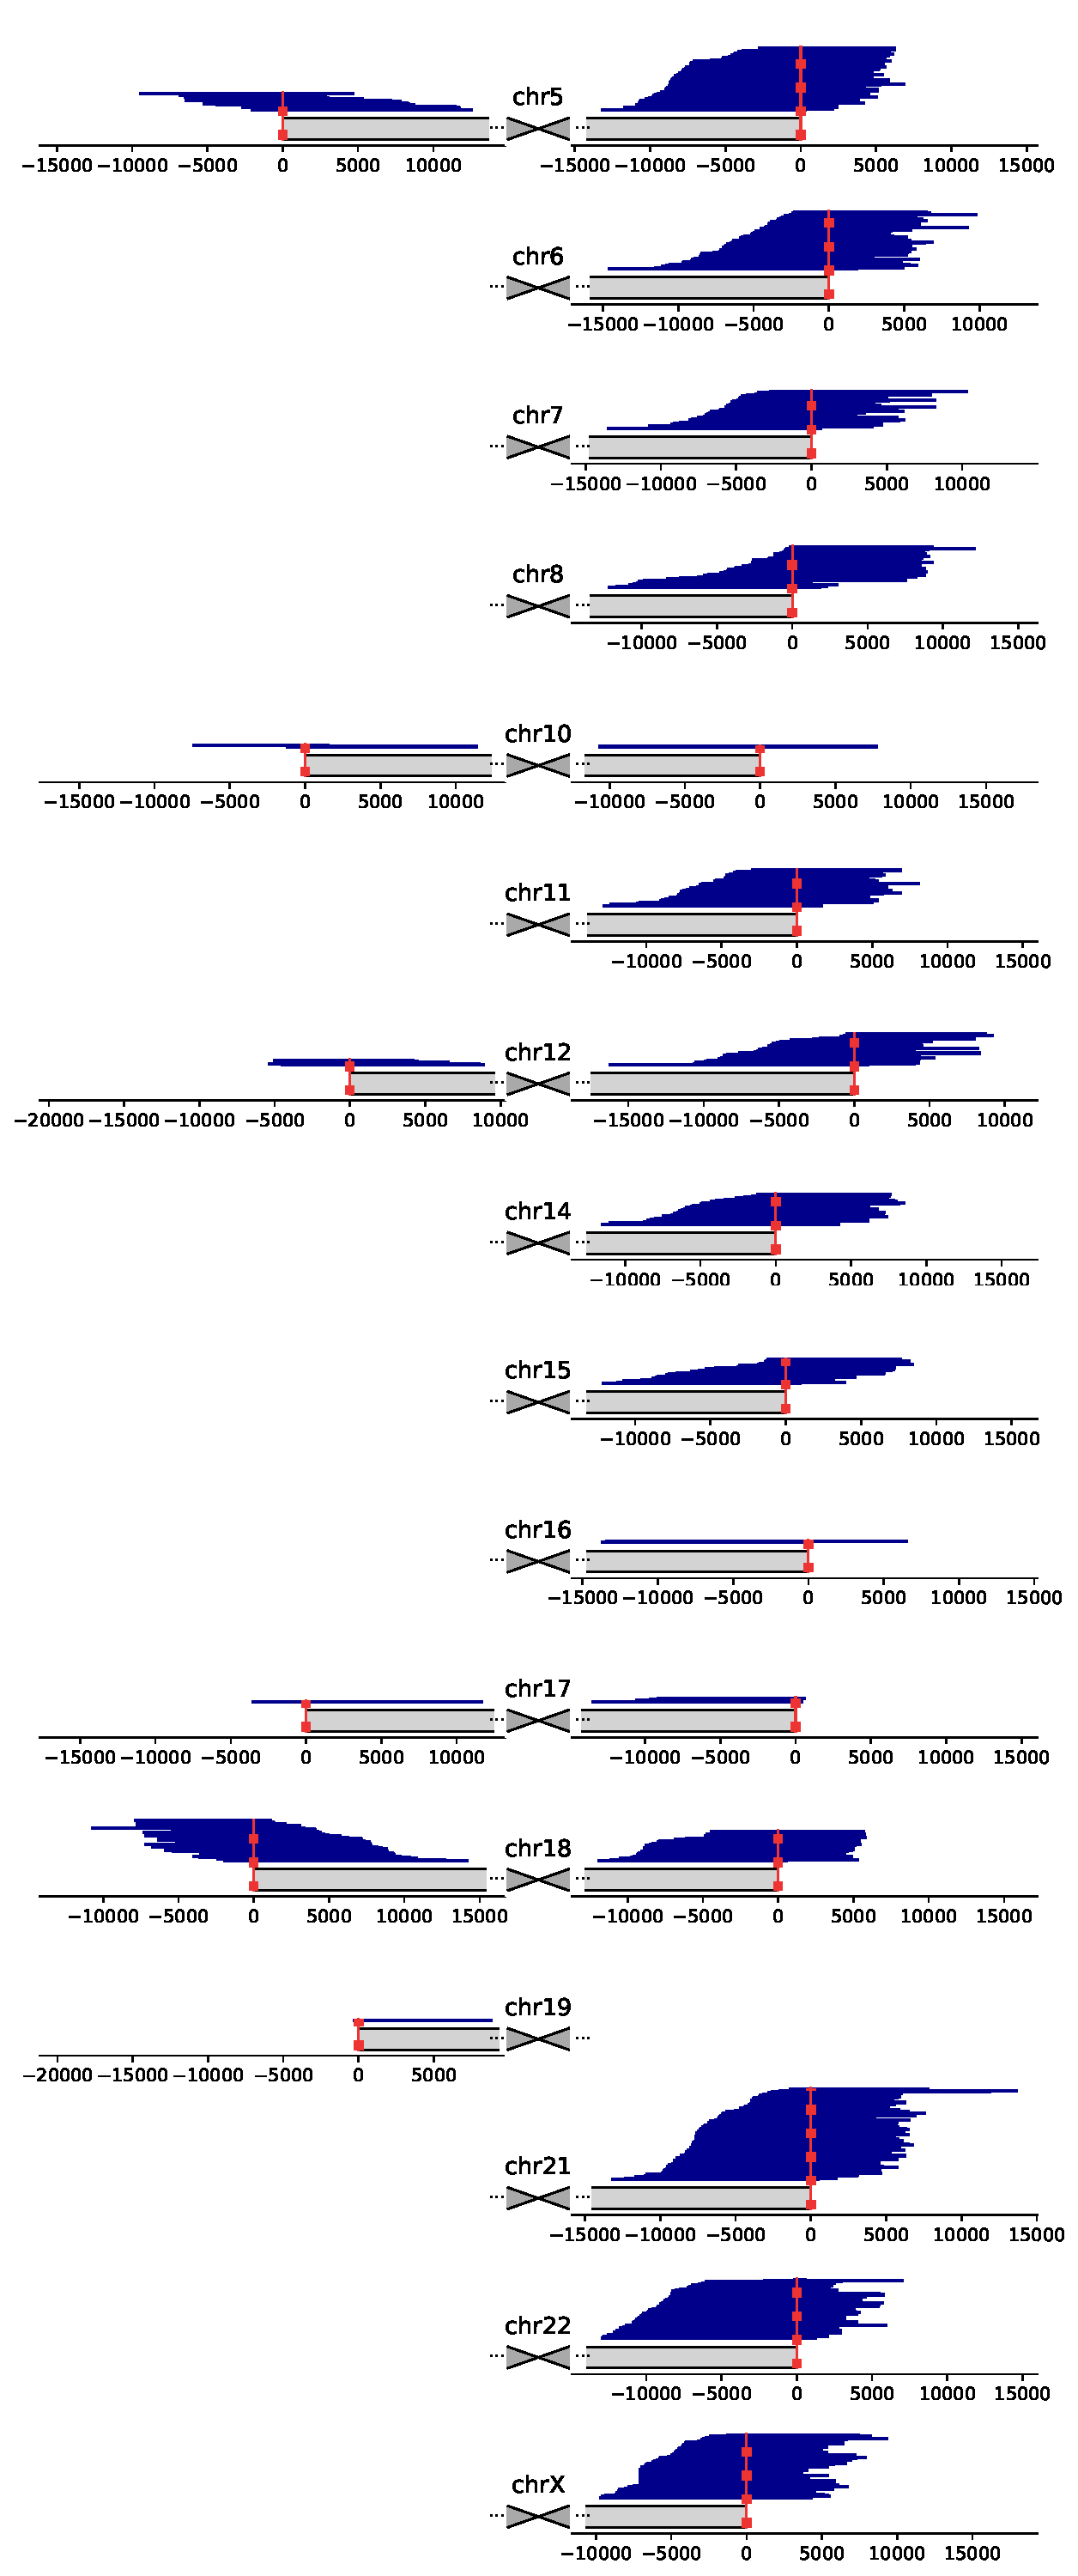
\includegraphics[height=.85\textheight,width=\textwidth,keepaspectratio]{figures/HG002-alignment.pdf}
% \caption{
%     Mapping of candidate telomeric PacBio CCS reads from the HG002 dataset.
%     Chromosomes are displayed schematically, centered around the centromere, with only the arms shown to which candidate reads aligned.
%     Vertical red dashed lines denote the position of the boundary of the annotated telomeric tract.
%     Coordinates are given in bp, relative to the positions of the telomeric tract boundaries.
% }
% \label{fig:hg002_alignment}
% \end{figure}
% \clearpage \pagebreak
% 
% %\addcontentsline{toc}{subsection}{\autoref{fig:hg002_densityplot_q_arm}}
% \begin{figure}[h!] \centering
% 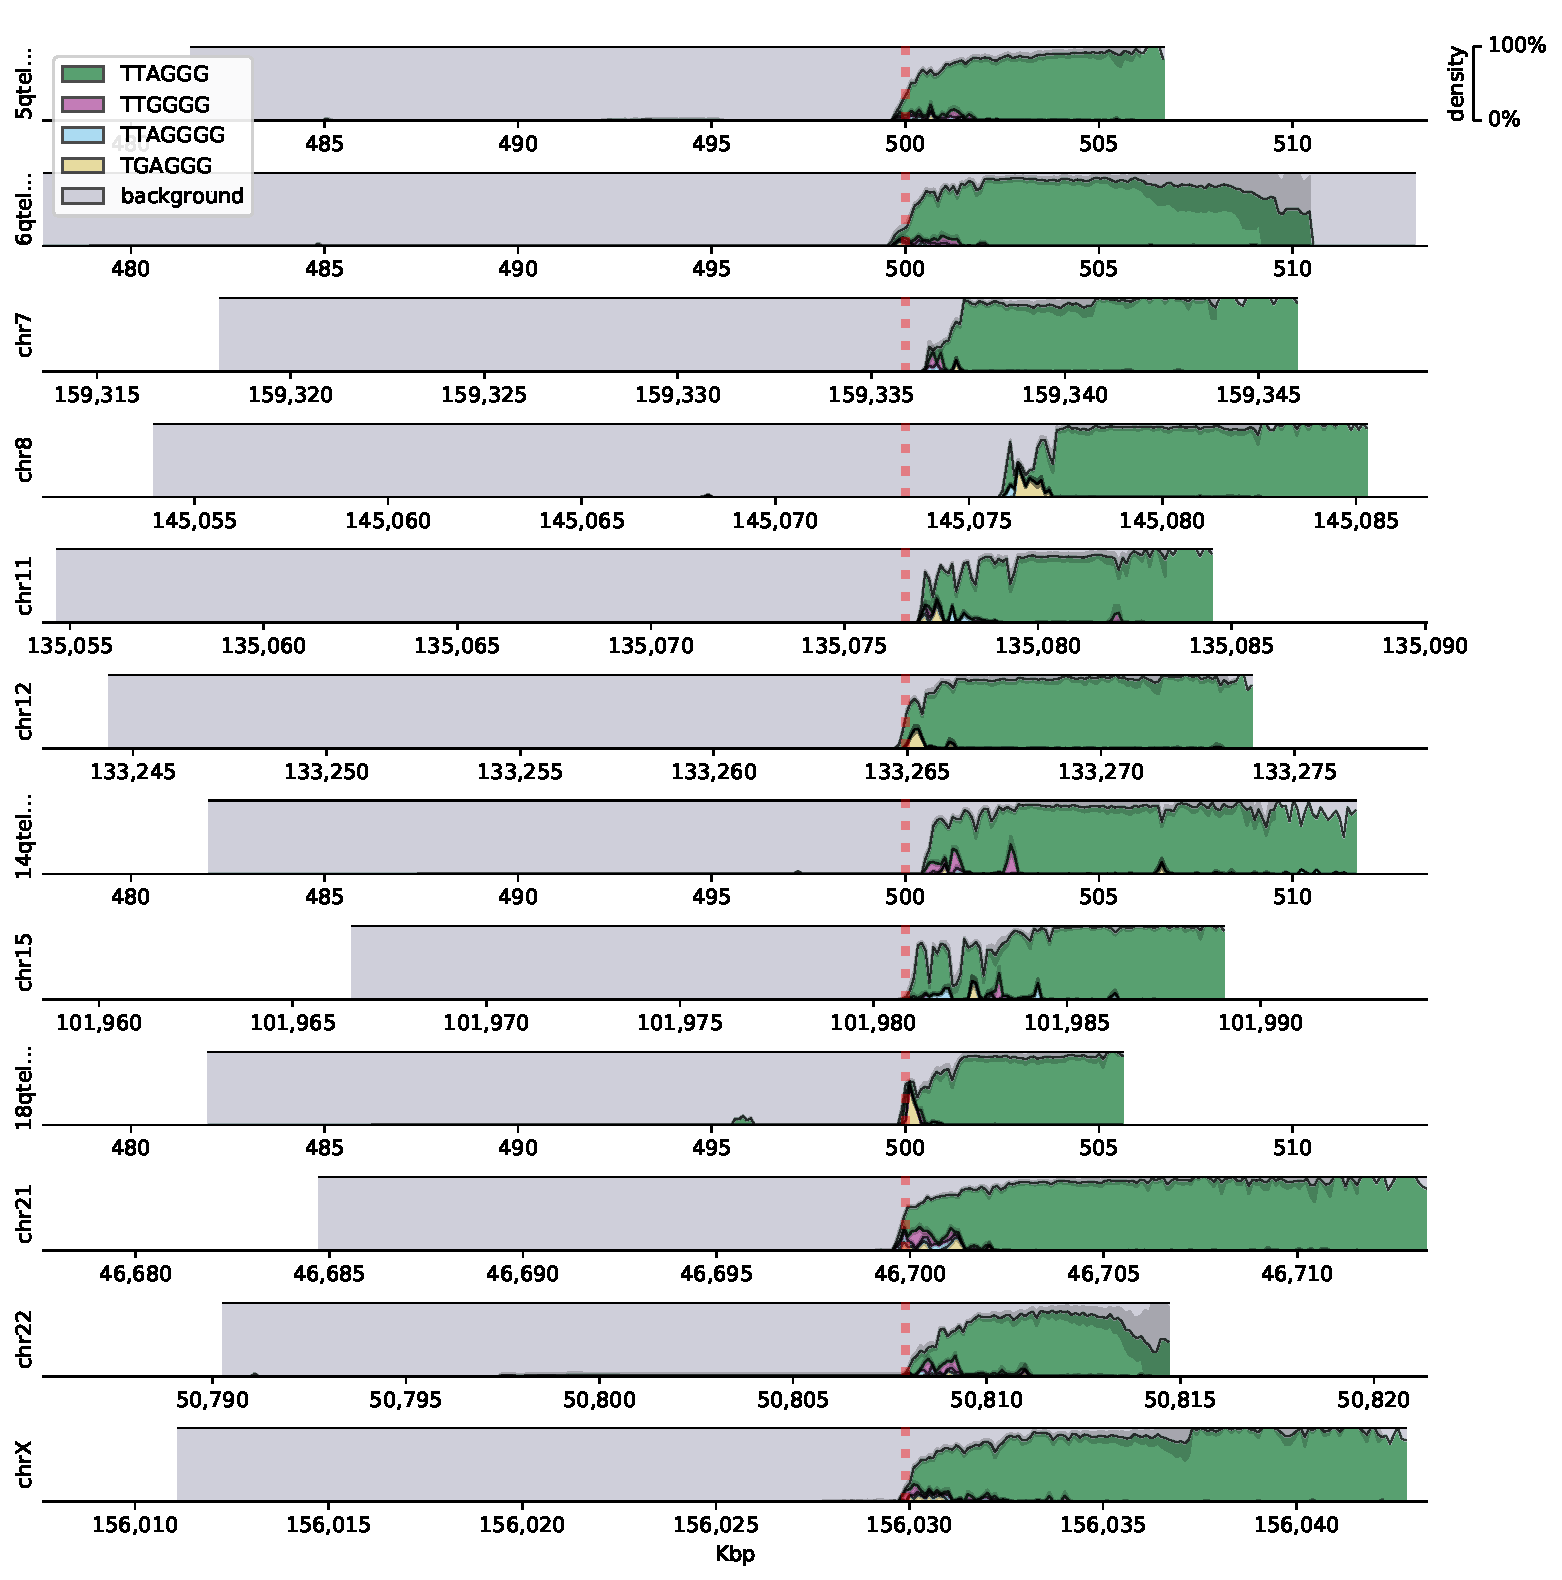
\includegraphics[height=\textheight,width=\textwidth,keepaspectratio]{figures/HG002-densityplot-q_arm.pdf}
% \caption{
%     Motif densities at ends of chromosomal \textit{q} arms of the HG002 dataset.
%     Only the arms covered by at least 20 reads are displayed.
%     Shaded boxes span the mapped regions of the genome.
%     Motif densities are plotted as stacked area charts; ribbons surrounding area boundaries represent the 95\% confidence interval of bootstrap.
%     Top four enriched motifs (contributing to at least 0.5\% of the repeat content) are plotted in color; pale tinted areas represent the density of any other motifs and non-repeating sequences (absence of enriched motifs).
%     Absolute genomic coordinates are given in Mbp on the specific reference contigs the reads mapped to (for example, for chr5, reads mapped to the 500 Kbp-long subtelomeric assembly \mbox{5qtel\_1-500K\_1\_12\_12}).
%     Vertical red dashed lines denote the position of the boundary of the annotated telomeric tract.
% }
% \label{fig:hg002_densityplot_q_arm}
% \end{figure}
% \clearpage \pagebreak
% 
% %\addcontentsline{toc}{subsection}{\autoref{fig:levenshtein_q_arm}}
% \begin{figure}[ht!] \centering
% 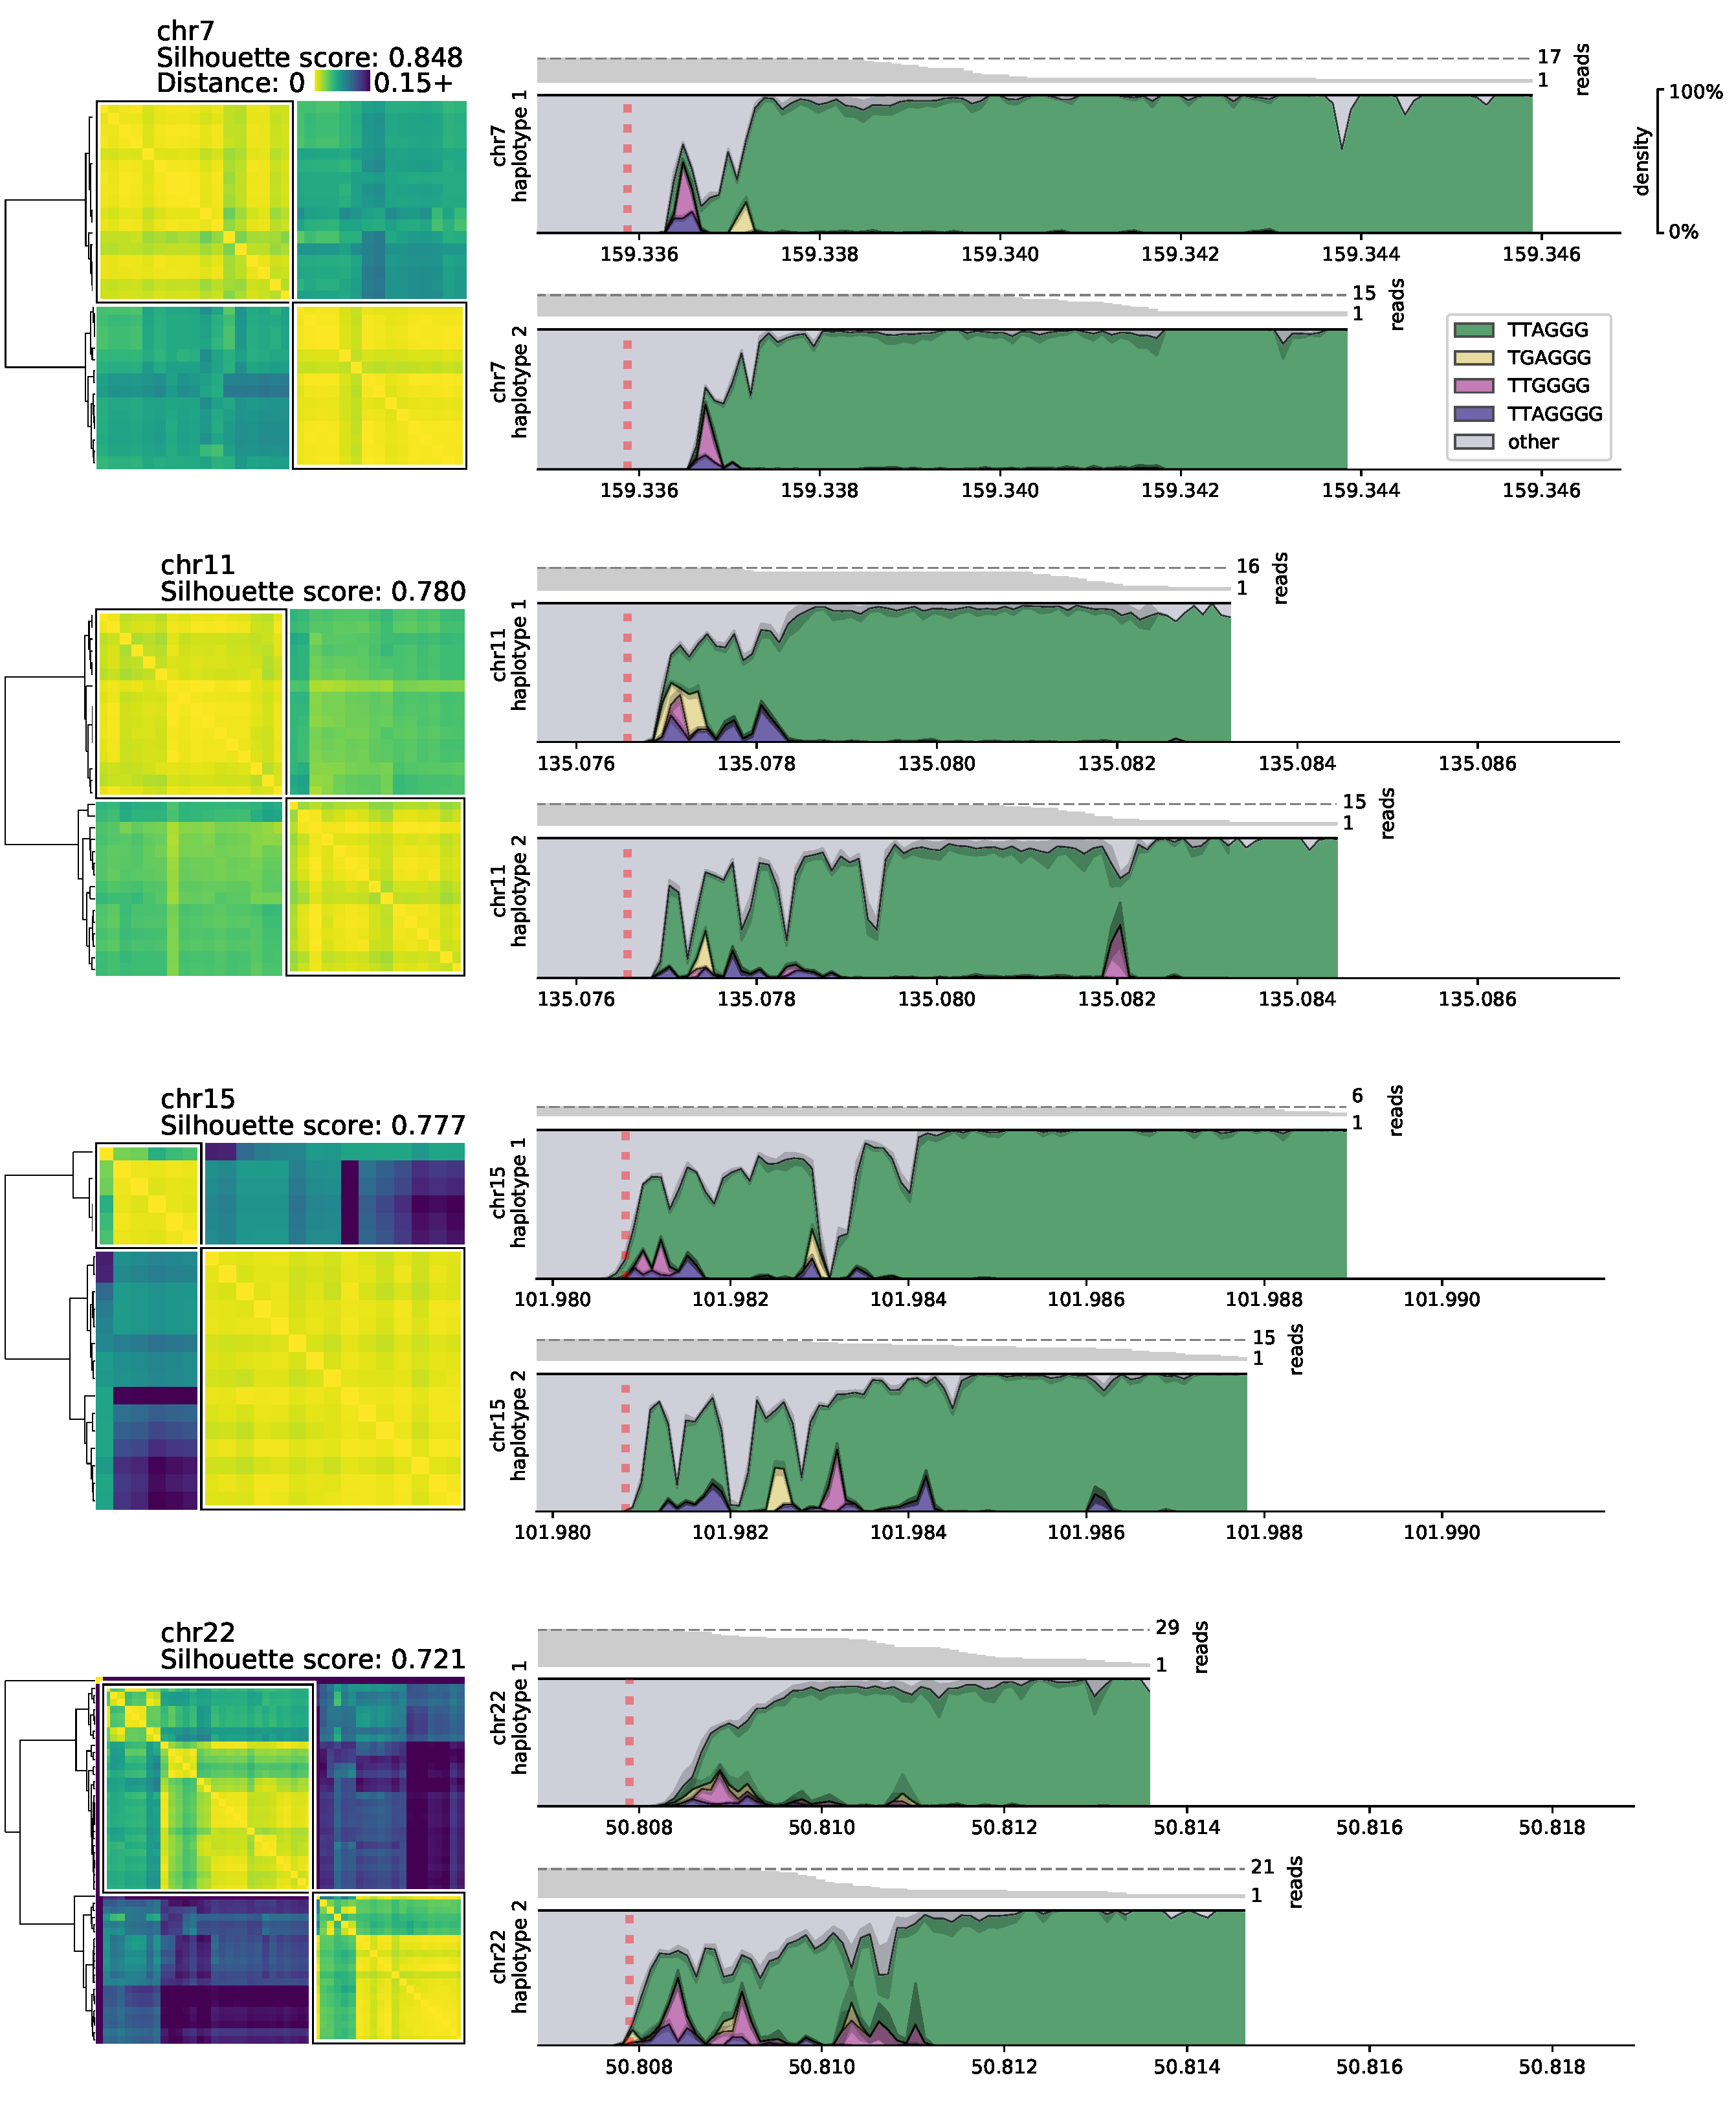
\includegraphics[height=.9\textheight,width=\textwidth,keepaspectratio]{figures/HG002-levenshtein-densityplots.pdf}
% \caption{
%     Clustering of reads into haplotypes based on relative pairwise Levenshtein distances on four representative chromosomal \textit{q} arms in the HG002 dataset, and densities of top enriched motifs in each haplotype.
%     Genomic coordinates are given in Mbp.
%     Read coverage of each haplotype is annotated above the density plot.
% }
% \label{fig:levenshtein_q_arm}
% \end{figure}
% \clearpage \pagebreak
% 
% \pagebreak
% \section*{Tables} \addcontentsline{toc}{section}{Tables}
% 
% \begin{samepage} \begin{table}[h!] \small \begin{tabular}{llllll}
\hline
\textbf{Motif}  & \textbf{Arm} & \multicolumn{3}{l}{\textbf{Abundance}}           & \textbf{Combined adjusted p-value} \\
\textbf{}       & \textbf{}    & \textbf{HG001} & \textbf{HG002} & \textbf{HG005} & \textbf{}                          \\
\hline
TTAGGG          & q            & 0.506392       &  0.432620      &  0.544289      &  0.00e+00                          \\
TGAGGG          & q            & 0.011527       &  0.017107      &  0.025117      &  8.33e-46                          \\
TTGGGG          & q            & 0.014520       &  0.021062      &  0.015897      &  2.13e-45                          \\
TTAGGGG         & q            & 0.014502       &  0.013954      &  0.015123      &  0.00e+00                          \\
TAGGG           & q            & 0.004637       &  0.003448      &  0.005159      &  4.46e-32                          \\
TTAGG           & q            & 0.004529       &  0.003182      &  0.004487      &  1.04e-30                          \\
TTTAGGG         & q            & 0.004508       &  0.003721      &  0.003078      &  7.95e-33                          \\
TTAGGGTTAGGGG   & q            & 0.004357       &  0.003782      &  0.004980      &  1.44e-38                          \\
TTAGGTTAGGG     & q            & 0.003650       &  0.002806      &  0.003548      &  4.97e-36                          \\
TAGGGTTAGGG     & q            & 0.003597       &  0.003075      &  0.004034      &  4.60e-37                          \\
TTGGG           & q            & 0.002112       &  0.000966      &  0.002253      &  3.79e-12                          \\
TTAAGGG         & q            & 0.001827       &  0.002942      &  0.002856      &  8.68e-26                          \\
TTGGGTTAGGG     & q            & 0.001317       &  0.000530      &  0.001532      &  3.67e-20                          \\
TTAGGGTTTAGGG   & q            & 0.001104       &  0.001442      &  0.001486      &  1.66e-22                          \\
TTAGGGTTAAGGG   & q            & 0.000490       &  0.001690      &  0.000495      &  1.00e-15                          \\
TTAGGGGG        & q            & 0.000358       &  0.001613      &  0.000526      &  0.00e+00                          \\
TTAGGGTTGTTAGGG & q            & 0.000272       &  0.000500      &  0.000438      &  2.13e-28                          \\
TTAGAGGG        & q            & 0.000146       &  0.000046      &  0.000103      &  4.72e-3                           \\
TTGGGGTTGGGGG   & q            & 0.000073       &  0.000095      &  0.000075      &  2.35e-7                           \\
TGGTTAGGGTTAGGG & q            & 0.000045       &  0.000208      &  0.000164      &  1.62e-12                          \\
CCCTAA          & p            & 0.099720       &  0.226981      &  0.188396      &  0.00e+00                          \\
CCCCAA          & p            & 0.010279       &  0.010869      &  0.007581      &  5.65e-31                          \\
CCCCTAA         & p            & 0.007083       &  0.007903      &  0.006217      &  8.83e-47                          \\
CCGCG           & p            & 0.002097       &  0.001710      &  0.002713      &  9.93e-40                          \\
CCCG            & p            & 0.000703       &  0.000330      &  0.000493      &  2.09e-31                          \\
GGGG            & p            & 0.000502       &  0.000122      &  0.000202      &  2.42e-22                          \\
TTTT            & p            & 0.000183       &  0.000109      &  0.000153      &  9.52e-17                          \\
\hline
\end{tabular}
\caption{Significantly enriched repeating motifs in telomeric regions of GIAB datasets HG001, HG002, and HG005.}
\label{tab:repeatfinder_full}
\end{table}
\end{samepage}

% \begin{samepage} \begin{table}[h!] \begin{tabular}{lll}
\hline
\textbf{Chromosome}             &  \textbf{Silhouette score}  &  \textbf{Mann-Whitney U adjusted p value}  \\  \hline
chr7                            &  0.848                      &  8.743e-82                                 \\
chr11                           &  0.780                      &  2.893e-76                                 \\
chr15                           &  0.777                      &  2.205e-34                                 \\
chr22                           &  0.721                      &  2.141e-206                                \\
14qtel\_1-500K\_1\_12\_12\_rc   &  0.711                      &  7.682e-48                                 \\
18qtel\_1-500K\_1\_12\_12\_rc   &  0.567                      &  3.844e-35                                 \\
chrX                            &  0.516                      &  1.075e-165                                \\
chr21                           &  0.498                      &  0.0                                       \\
chr12                           &  0.483                      &  3.306e-36                                 \\
6qtel\_1-500K\_1\_12\_12\_rc    &  0.418                      &  2.550e-122                                \\
5qtel\_1-500K\_1\_12\_12\_rc    &  0.387                      &  9.768e-131                                \\
chr8                            &  0.312                      &  6.722e-19                                 \\
\hline
\end{tabular}
\caption{Silhouette scores for cluster assignments on \textit{q} arms of chromosomes in sample HG002 where two clusters of reads are present, and adjusted \textit{p}-values for the Mann-Whitney U test for the difference of within-cluster and out-of-cluster relative pairwise Levenshtein distances.}
\label{tab:levenshtein-q_arm}
\end{table}
\end{samepage}


%%%%%%%%%%%%%%%%%%%%%%%%%%%%%%%%%%%%%%%%%%%%%%%%%%%%%%%%%%%%%%%%%%%%%%%%%%%%%%%%

% \beginsupplement
% 
% \singlespacing
% \addcontentsline{toc}{section}{Supplemental materials}
% \begin{center}
%     \LARGE{\textbf{Haplotype Diversity and Sequence Heterogeneity of Human Telomeres}}
%     \\~\\
%     \small{Kirill Grigorev, Jonathan Foox \textit{et al.}}
% \section*{Supplemental materials}
% \end{center}
% \doublespacing
% 
% \subsection*{Supplemental methods} \addcontentsline{toc}{subsection}{Supplemental methods} \label{sec:supp_methods}
% 
% To test the presence of non-canonical repeat motifs in datasets generated by technologies other than SMRT,
% we generated four whole-genome Illumina datasets (mean coverage $\sim$104x)
% and three linked-read 10X datasets (mean coverage $\sim$28x)
% for one individual at different timepoints aboard the International Space Station (ISS),
% and one additional linked-read 10X dataset (coverage $\sim$47x) for another individual aboard the ISS.
% From these datasets, candidate telomeric short reads were selected using \textit{Telomerecat} \cite{telomerecat},
% and enriched repeated motifs were discovered \textit{de novo} with the method described in \hyperref[sec:methods]{Materials and Methods}.
% \textit{p}-values were combined with the Mudholkar-George method \cite{george} within each technology (Illumina, 10X),
% and the Bonferroni multiple testing correction was applied
% (note: the Bonferroni correction was applied simultaneously to the \textit{p}-values for the motifs in PacBio reads (\autoref{tab:repeatfinder_full}) and for the motifs in short and linked reads).
% Motifs that were significantly enriched (adjusted \textit{p}-value below the cutoff of 0.05) in the datasets produced by all three technologies (PacBio, Illumina, 10X), with respect to reverse-complemented equivalence, were reported (\autoref{tab:shortread_repeatfinder}).
% 
% \pagebreak
% 
% \subsection*{Supplemental figures} \addcontentsline{toc}{subsection}{Supplemental figures} \label{sec:supp_figs}
% 
% \begin{figure}[ht!] \centering
% 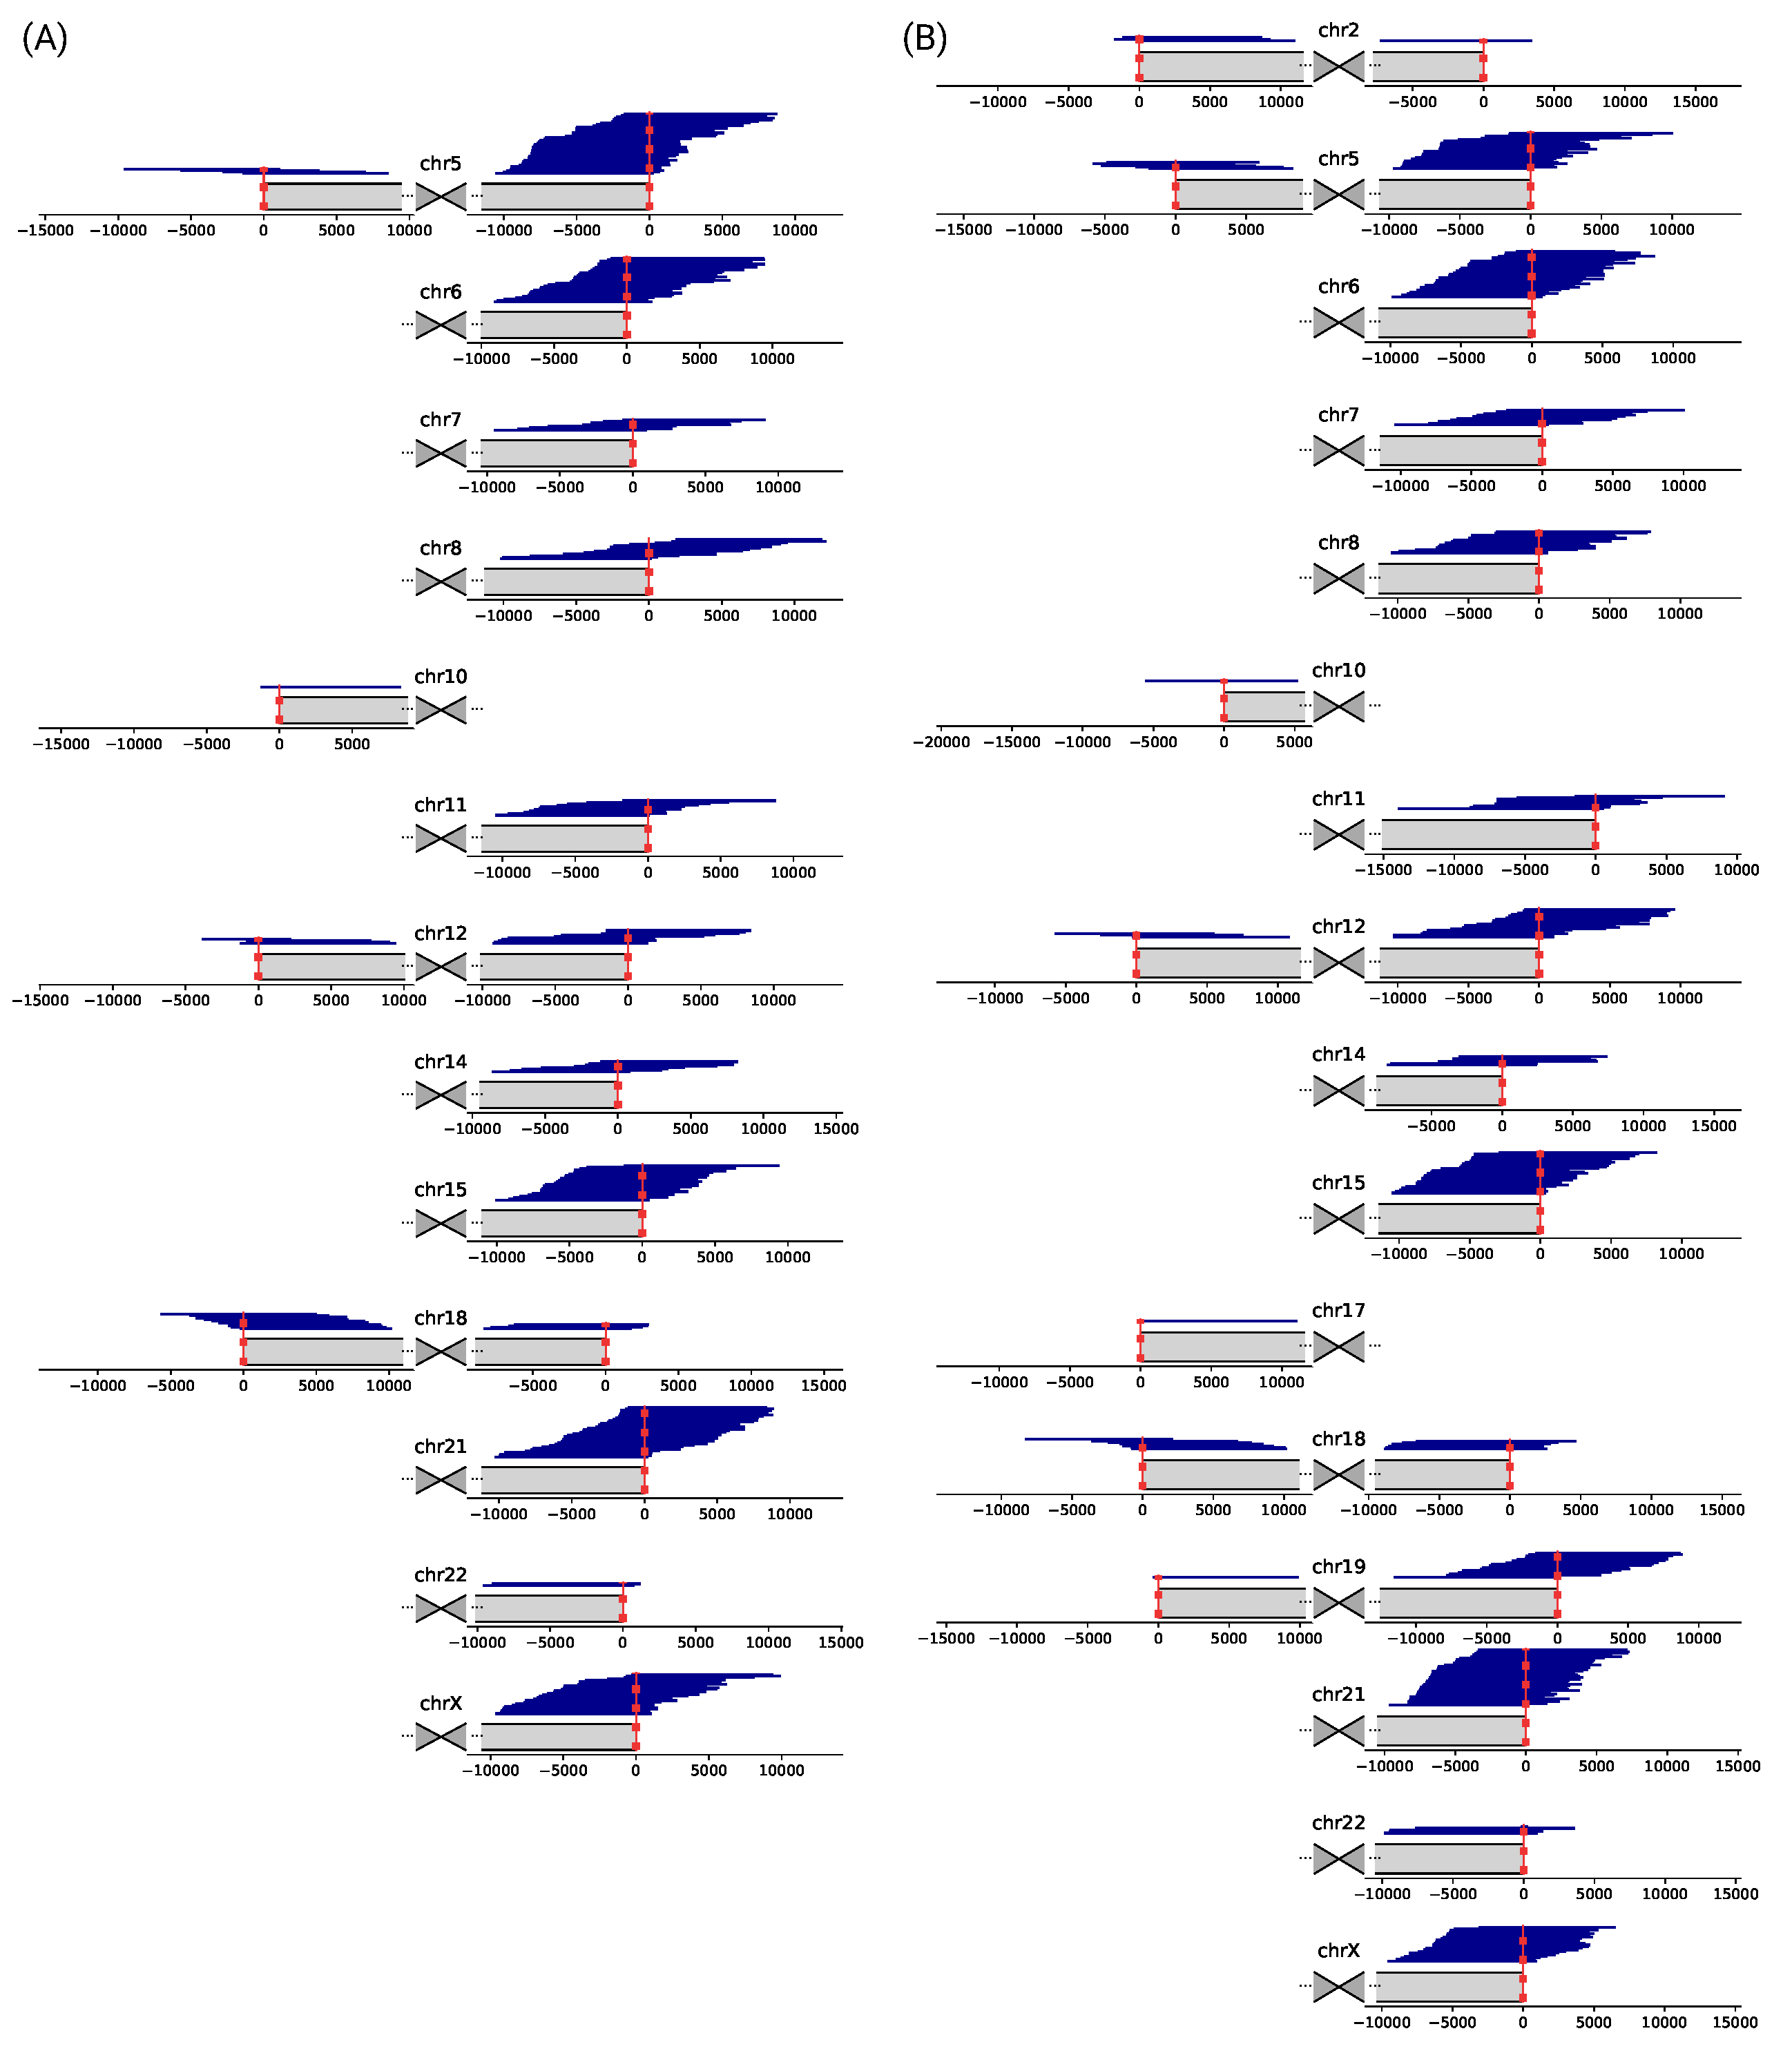
\includegraphics[height=.65\textheight,width=\textwidth,keepaspectratio]{figures/HG00X-alignments.pdf}
% \caption{
%     Mapping of candidate telomeric PacBio CCS reads from datasets (A) HG001 and (B) HG005.
%     Chromosomes are displayed schematically, centered around the centromere, with only the arms shown to which candidate reads aligned.
%     Vertical red dashed lines denote the position of the boundary of the annotated telomeric tract.
%     Coordinates are given in bp, relative to the positions of the telomeric tract boundaries.
% }
% \label{fig:hg00x_alignments}
% \end{figure}
% \clearpage \pagebreak
% 
% \begin{figure}[ht!] \centering
% 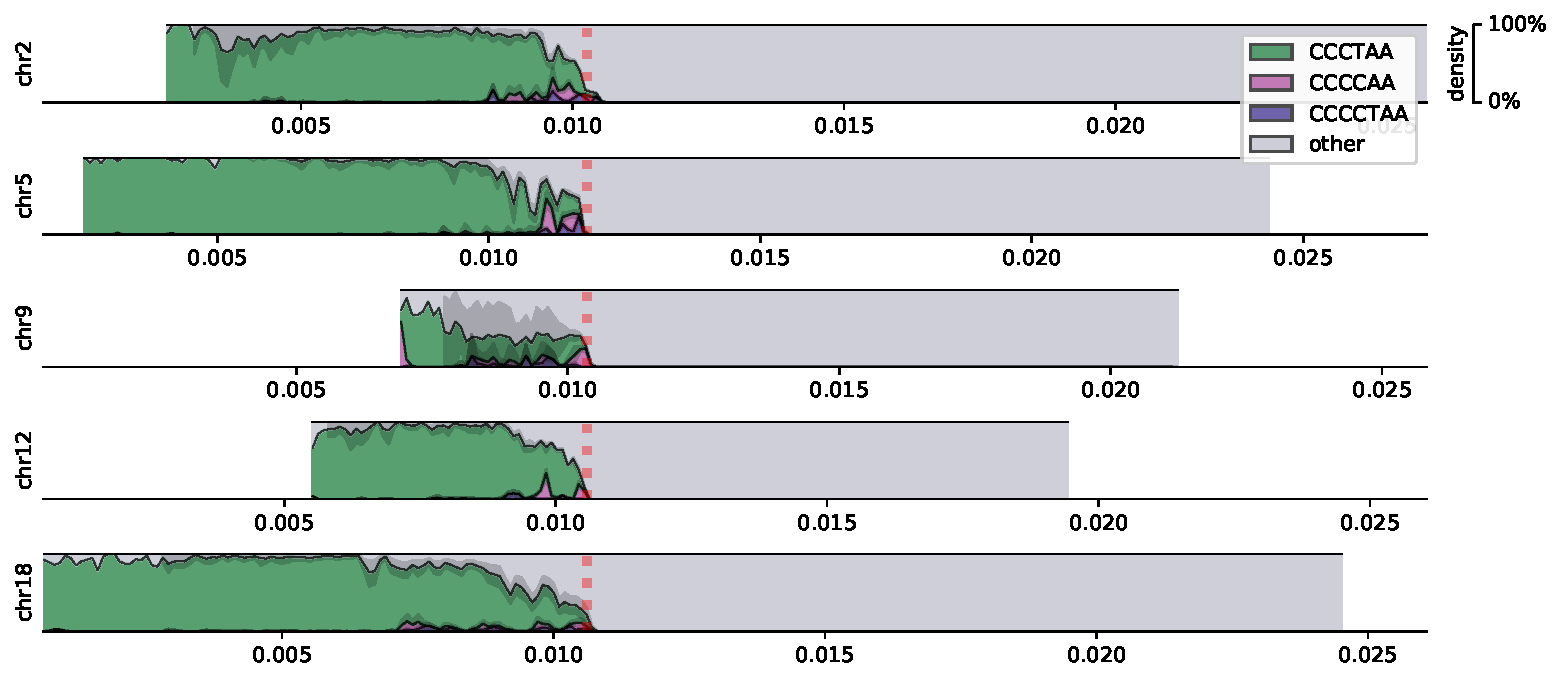
\includegraphics[height=.9\textheight,width=\textwidth,keepaspectratio]{figures/threemotifp/HG002-densityplot-p_arm-threemotifp.pdf}
% \caption{
%     Densities of top three enriched motifs (contributing to at least 0.5\% of the repeat content) at ends of chromosomal \textit{p} arms of the HG002 dataset.
%     Only the arms covered by at least 20 reads are displayed.
%     Genomic coordinates are given in Mbp.
%     Vertical red dashed lines denote the position of the boundary of the annotated telomeric tract.
% }
% \label{fig:hg002_densityplot_p_arm}
% \end{figure}
% \clearpage \pagebreak
% 
% \begin{figure}[ht!] \centering
% 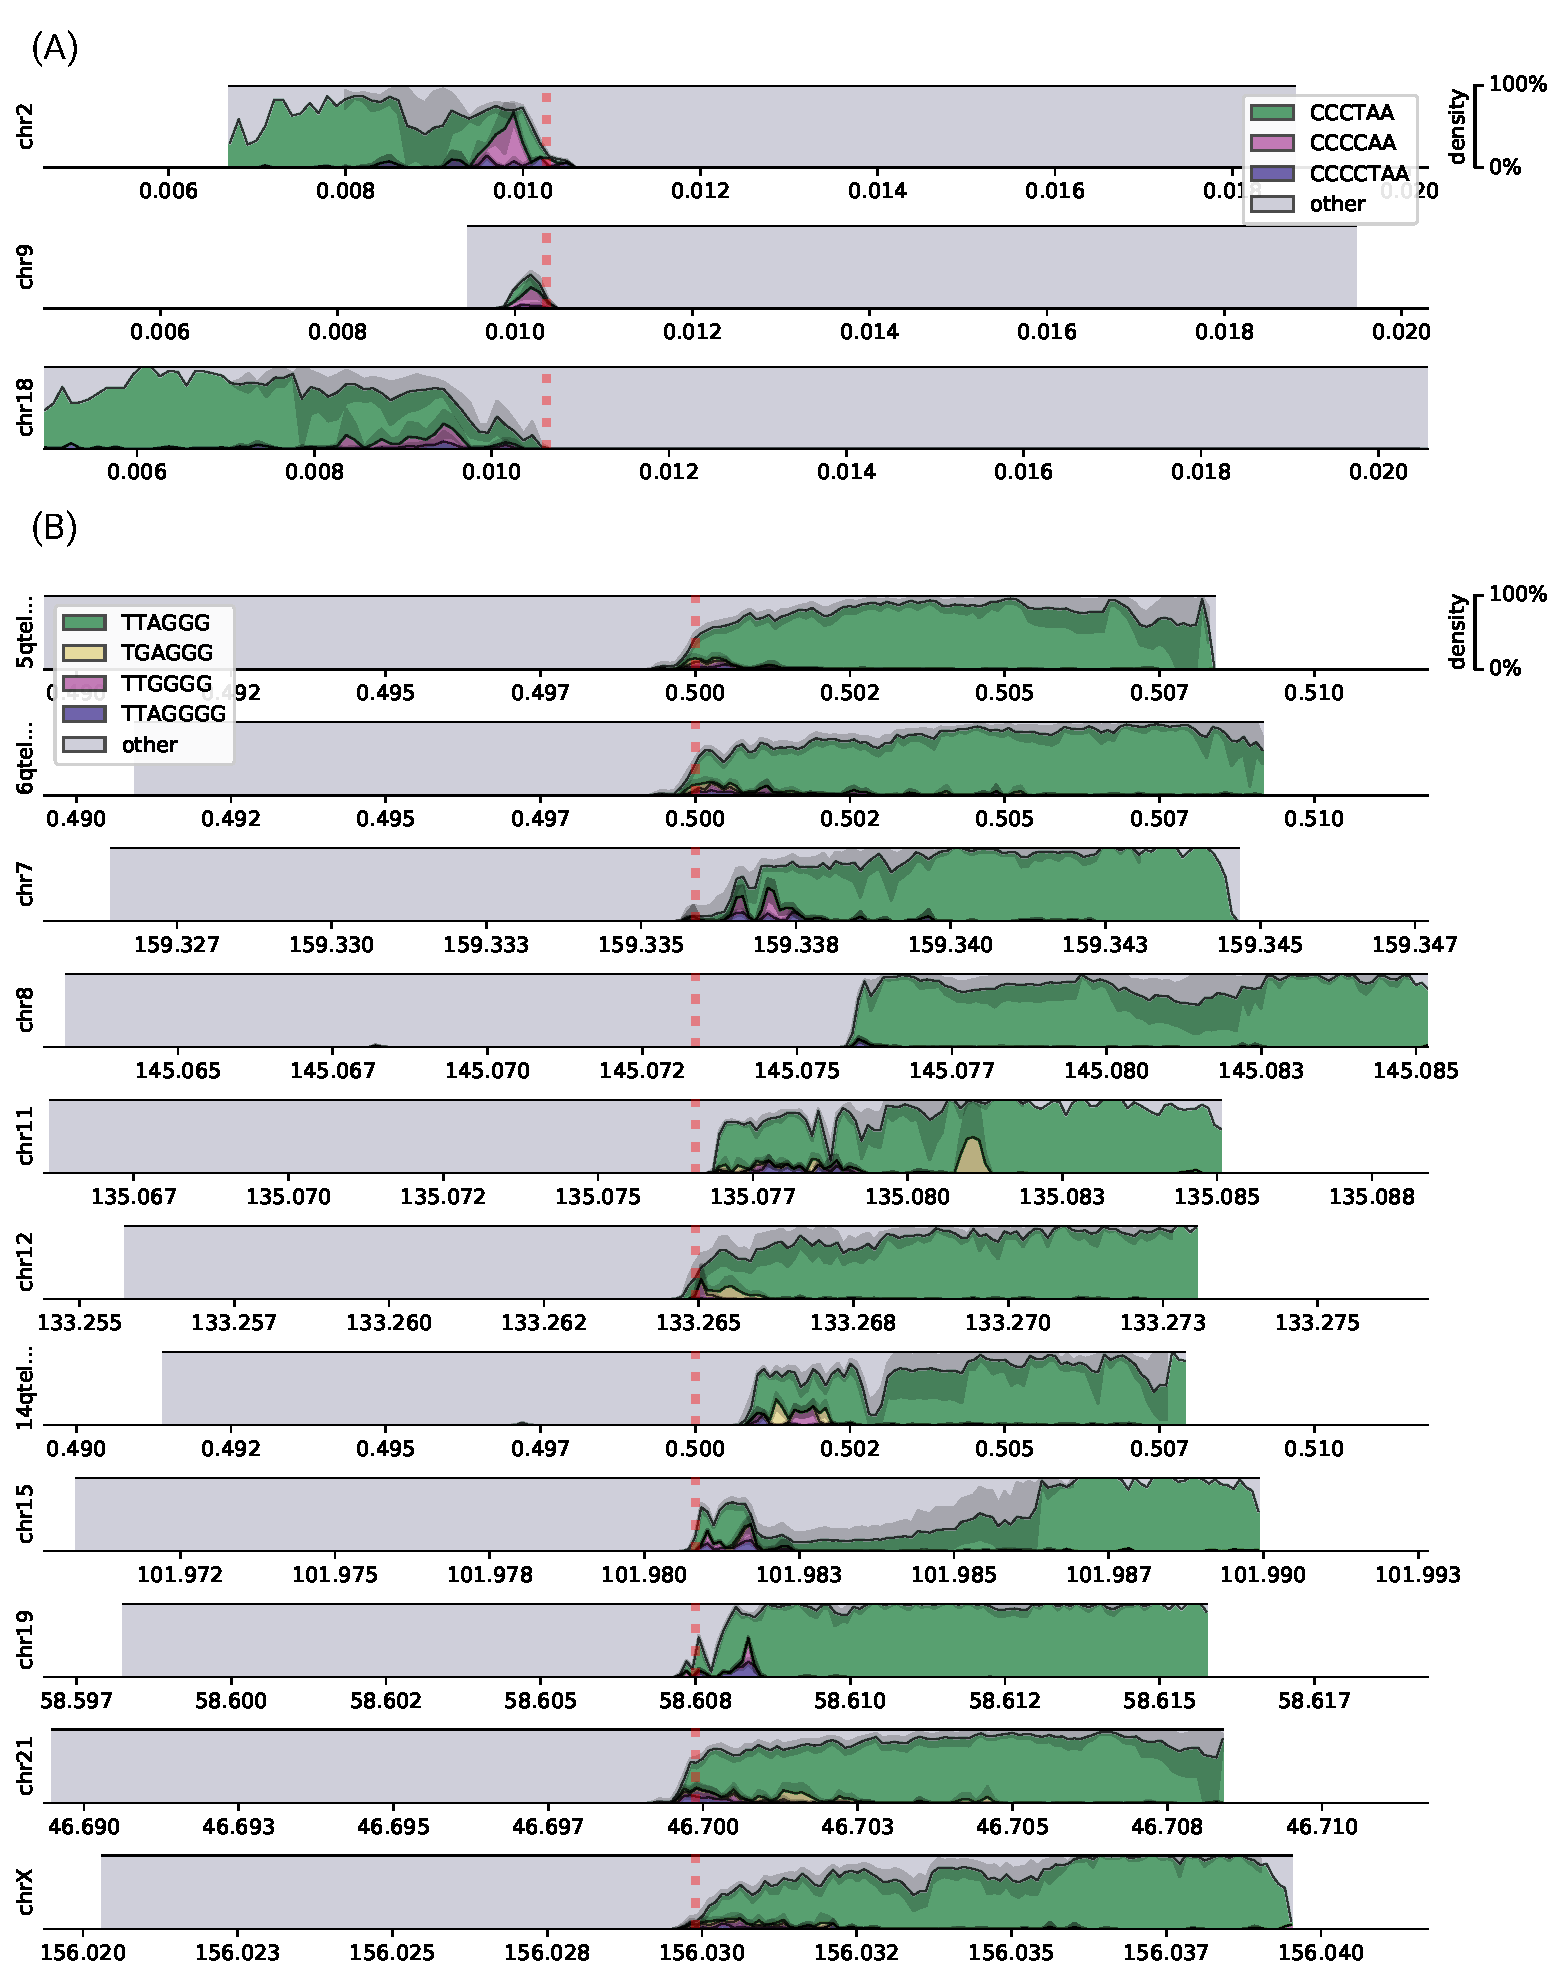
\includegraphics[height=.95\textheight,width=\textwidth,keepaspectratio]{figures/threemotifp/HG001-densityplots-threemotifp.pdf}
% \caption{
%     Motif densities at ends of chromosomal (A) \textit{p} and (B) \textit{q} arms of the HG001 dataset.
%     Only the arms covered by at least 20 reads are displayed.
%     Genomic coordinates are given in Mbp.
% }
% \label{fig:hg001_densityplots}
% \end{figure}
% \clearpage \pagebreak
% 
% \begin{figure}[ht!] \centering
% 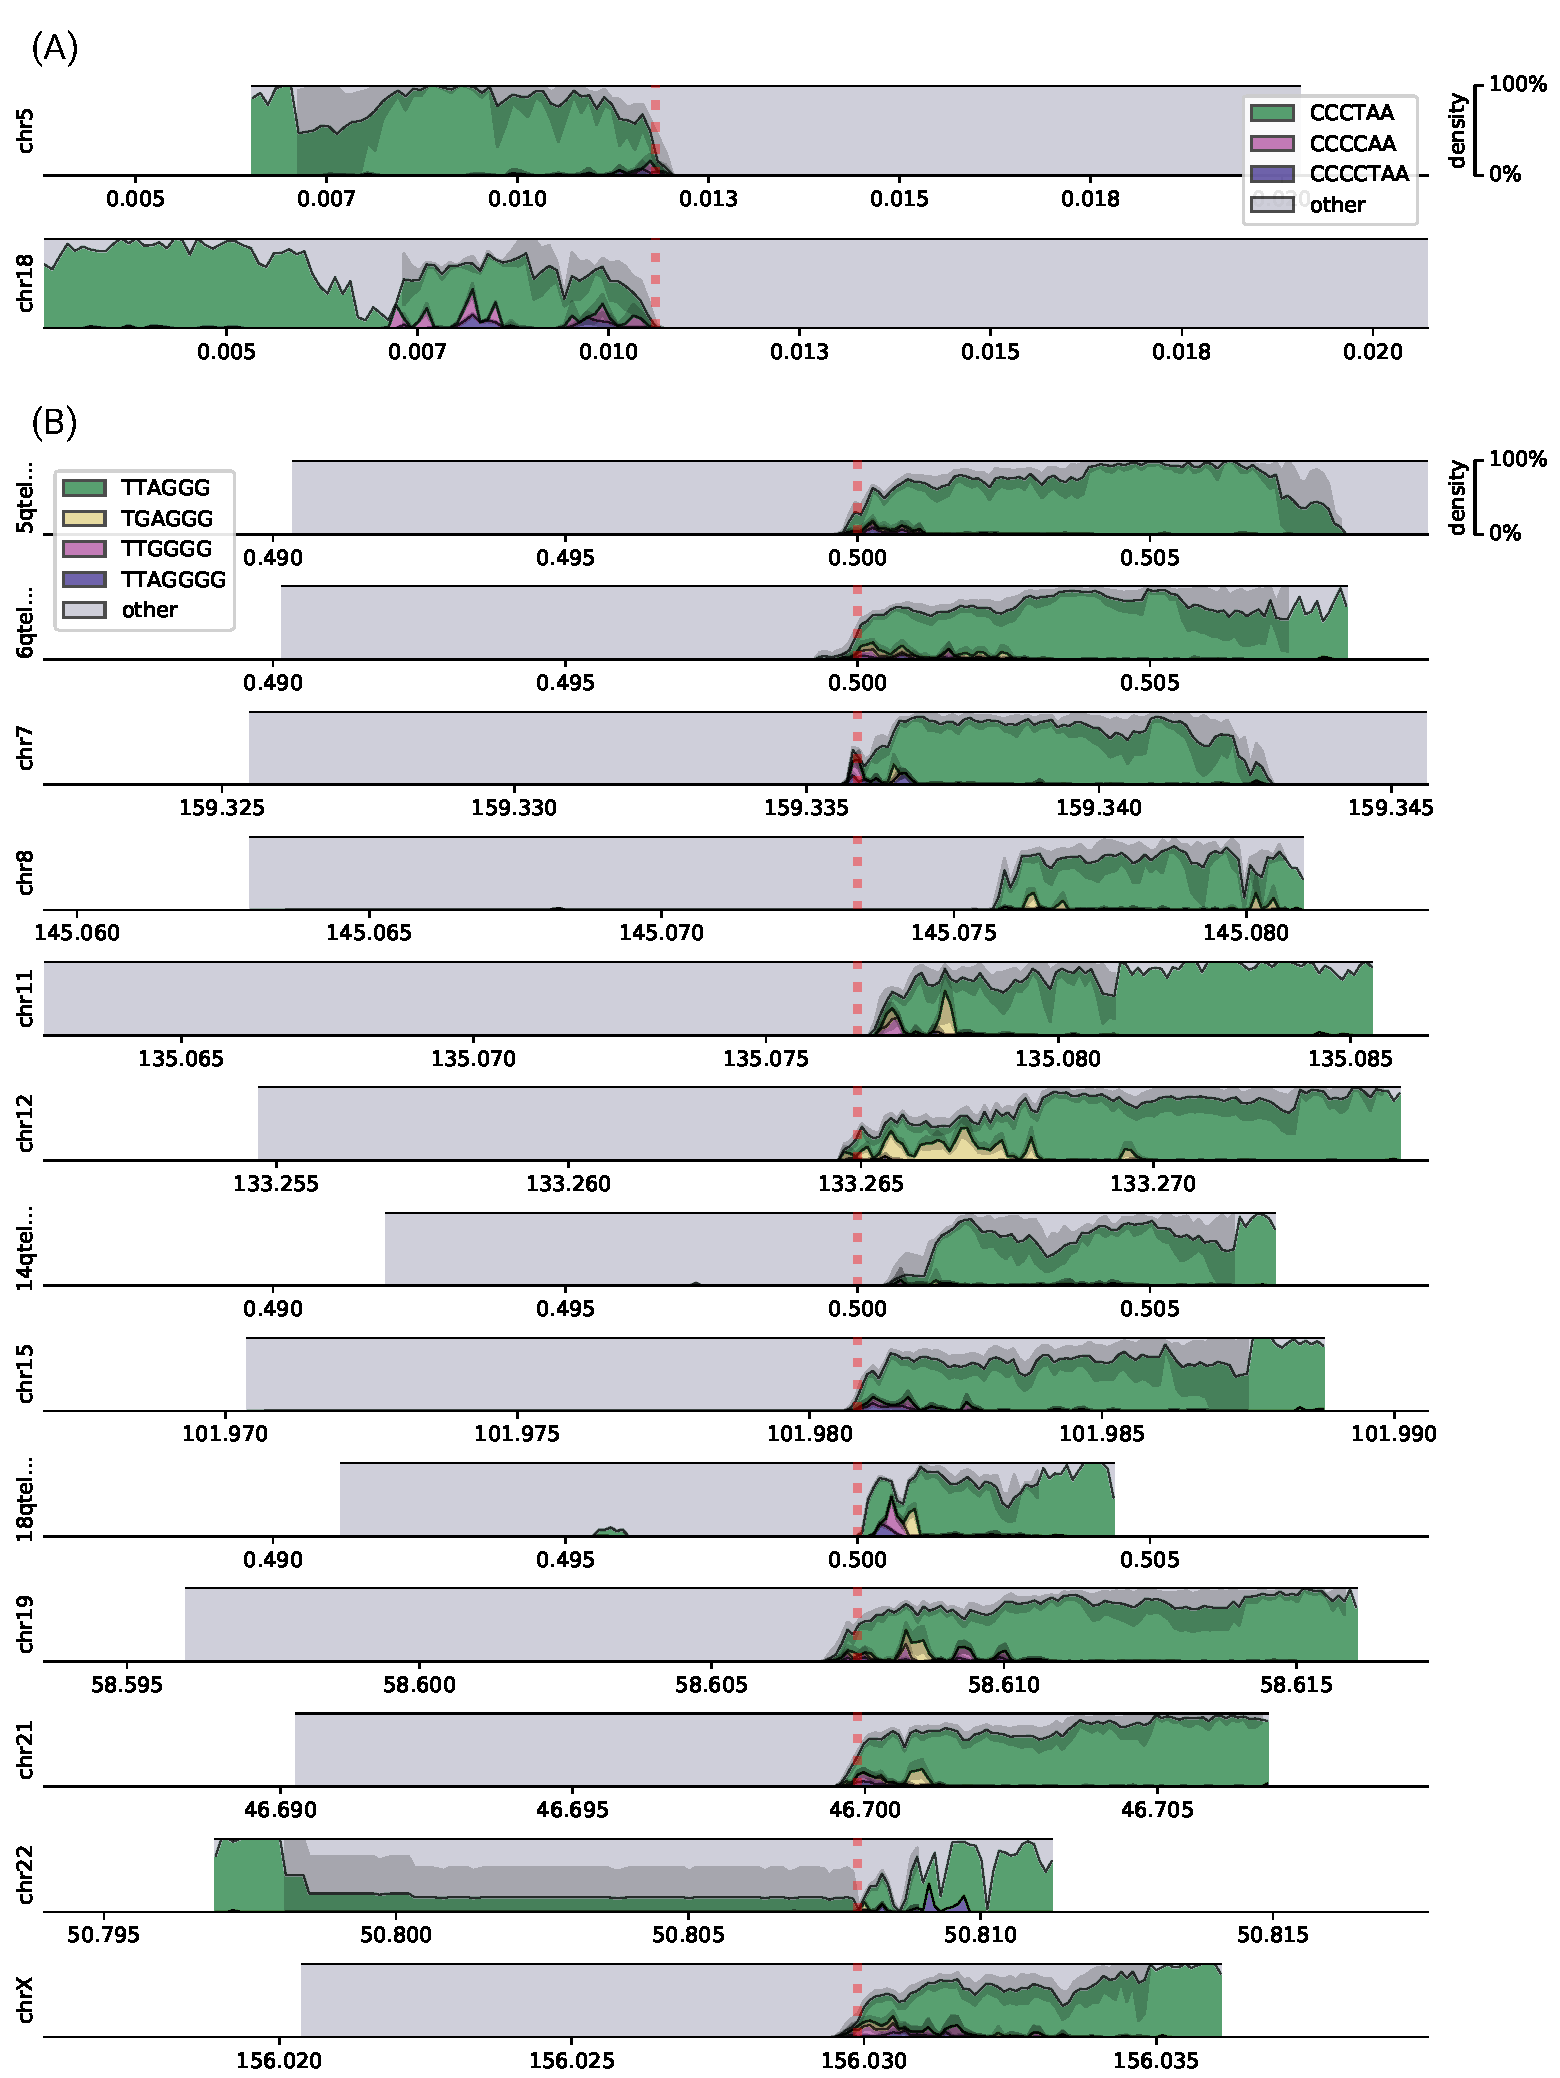
\includegraphics[height=.95\textheight,width=\textwidth,keepaspectratio]{figures/threemotifp/HG005-densityplots-threemotifp.pdf}
% \caption{
%     Motif densities at ends of chromosomal (A) \textit{p} and (B) \textit{q} arms of the HG005 dataset.
%     Only the arms covered by at least 20 reads are displayed.
%     Genomic coordinates are given in Mbp.
% }
% \label{fig:hg005_densityplots}
% \end{figure}
% \clearpage \pagebreak
% 
% \begin{figure}[ht!] \centering
% 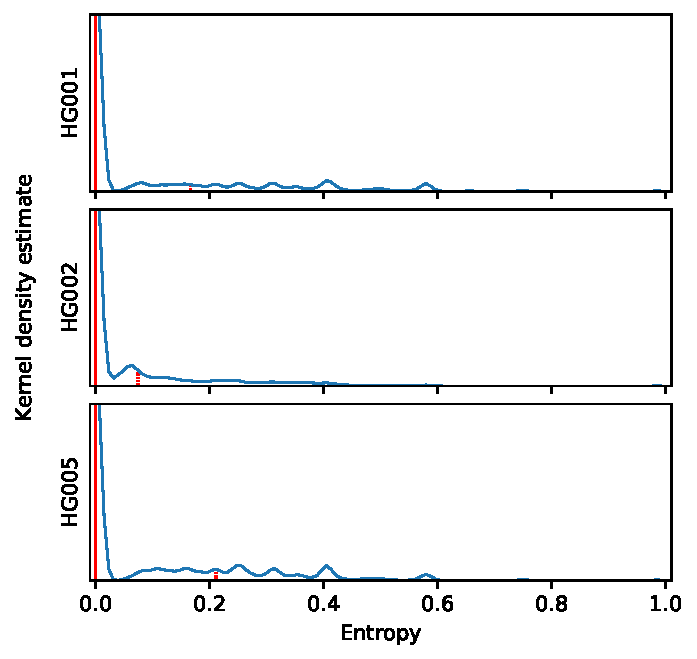
\includegraphics[height=.95\textheight,width=.65\textwidth,keepaspectratio]{figures/entropy.pdf}
% \caption{
%     Distribution of motif entropies in 10 bp windows of candidate PacBio CCS reads aligning to the same chromosomal arms in GIAB datasets HG001, HG002, and HG005.
%     Red solid lines denote the position of the median (0.000 in all three datasets), and red dashed lines denote the 3rd quartile (0.166, 0.074, and 0.211, respectively).
% }
% \label{fig:entropy}
% \end{figure}
% \clearpage \pagebreak
% 
% \subsection*{Supplemental tables} \addcontentsline{toc}{subsection}{Supplemental tables}
% \begin{samepage} \begin{table}[h!] \begin{tabular}{llllll}
\hline
\textbf{chromosome}  &  \textbf{reference contig}        &  \textbf{arm}  &  \textbf{HG001}  &  \textbf{HG002}  &  \textbf{HG005} \\
\hline
chr2                 &  2qtel\_1-500K\_1\_12\_12\_rc     &  q             &  0               &  0               &  1              \\
chr2                 &  chr2                             &  p             &  5               &  16              &  3              \\
chr5                 &  5qtel\_1-500K\_1\_12\_12\_rc     &  q             &  42              &  53              &  23             \\
chr5                 &  chr5                             &  p             &  4               &  15              &  5              \\
chr6                 &  6qtel\_1-500K\_1\_12\_12\_rc     &  q             &  31              &  49              &  29             \\
chr7                 &  chr7                             &  q             &  8               &  32              &  10             \\
chr8                 &  chr8                             &  q             &  14              &  35              &  14             \\
chr9                 &  chr9                             &  p             &  6               &  6               &  0              \\
chr10                &  10qtel\_1-500K\_1\_12\_12\_rc    &  q             &  0               &  1               &  0              \\
chr10                &  chr10                            &  p             &  1               &  2               &  1              \\
chr11                &  chr11                            &  q             &  11              &  31              &  9              \\
chr12                &  chr12                            &  q             &  10              &  27              &  18             \\
chr12                &  chr12                            &  p             &  4               &  5               &  3              \\
chr14                &  14qtel\_1-500K\_1\_12\_12\_rc    &  q             &  8               &  26              &  6              \\
chr15                &  chr15                            &  q             &  25              &  21              &  26             \\
chr16                &  16qtel\_1-500K\_1\_12\_12\_rc    &  q             &  0               &  2               &  0              \\
chr16                &  chr16                            &  p             &  1               &  0               &  0              \\
chr17                &  17qtel\_1-500K\_1\_12\_12v2\_rc  &  q             &  0               &  4               &  0              \\
chr17                &  17ptel\_1\_500K\_1\_12\_12       &  p             &  0               &  1               &  1              \\
chr18                &  18qtel\_1-500K\_1\_12\_12\_rc    &  q             &  4               &  26              &  6              \\
chr18                &  chr18                            &  p             &  11              &  35              &  7              \\
chr19                &  19ptel\_1-500K\_1\_12\_12        &  p             &  0               &  1               &  1              \\
chr19                &  chr19                            &  q             &  6               &  0               &  16             \\
chr21                &  chr21                            &  q             &  35              &  77              &  35             \\
chr22                &  chr22                            &  q             &  2               &  51              &  5              \\
chrX                 &  chrX                             &  q             &  28              &  54              &  22             \\
\hline
\end{tabular}
\caption{The number of telomeric reads on each arm identified in GIAB PacBio CCS datasets HG001, HG002, and HG005.}
\label{tab:telomeric_read_counts}
\end{table}
\end{samepage}

% \begin{samepage} \begin{table}[h!] \small \begin{tabular}{lllll}
\hline
\textbf{Motif}  & \multicolumn{2}{l}{\textbf{Illumina datasets}}        & \multicolumn{2}{l}{\textbf{10X datasets}}             \\
\textbf{}       & \textbf{Median abundance} & \textbf{Adjusted p-value} & \textbf{Median abundance} & \textbf{Adjusted p-value} \\
\hline
TTAGGG          & 0.299068                  & 0.00e+0                   & 0.461711              & 0.00e+0                       \\
TGAGGG          & 0.007484                  & 0.00e+0                   & 0.018524              & 0.00e+0                       \\
TTGGGG          & 0.002495                  & 0.00e+0                   & 0.007190              & 0.00e+0                       \\
GGGG            & 0.020347                  & 0.00e+0                   & 0.006080              & 0.00e+0                       \\
TTAGGGG         & 0.003007                  & 0.00e+0                   & 0.005024              & 0.00e+0                       \\
TTTT            & 0.001294                  & 0.00e+0                   & 0.001490              & 0.00e+0                       \\
TTAAGGG         & 0.000664                  & 1.39e-55                  & 0.001124              & 1.58e-59                      \\
TTAGGGGTTAGGG   & 0.000533                  & 1.04e-51                  & 0.001020              & 0.00e+0                       \\
TAGGG           & 0.000619                  & 0.00e+0                   & 0.001020              & 0.00e+0                       \\
TTGGG           & 0.000500                  & 0.00e+0                   & 0.000989              & 0.00e+0                       \\
TTTAGGG         & 0.000622                  & 6.40e-55                  & 0.000884              & 1.02e-57                      \\
TAGGGTTAGGG     & 0.000312                  & 4.24e-40                  & 0.000503              & 0.00e+0                       \\
TTAGGGTTTAGGG   & 0.000176                  & 4.41e-38                  & 0.000284              & 6.22e-59                      \\
TTAGGGTTAAGGG   & 0.000145                  & 6.63e-36                  & 0.000264              & 4.15e-57                      \\
TTAGG           & 0.000241                  & 8.13e-35                  & 0.000213              & 1.10e-55                      \\
TTGGGTTAGGG     & 0.000127                  & 4.47e-28                  & 0.000178              & 3.34e-56                      \\
TTAGGGTTAGG     & 0.000066                  & 1.99e-18                  & 0.000092              & 7.82e-48                      \\
TTAGGGGG        & 0.000039                  & 1.02e-14                  & 0.000062              & 4.31e-40                      \\
TTAGGGTTGTTAGGG & 0.000035                  & 4.64e-09                  & 0.000061              & 4.65e-57                      \\
TTAGAGGG        & 0.000036                  & 5.44e-13                  & 0.000053              & 2.66e-36                      \\
TTGGGGTTGGGGG   & 0.000002                  & 4.51e-13                  & 0.000014              & 5.84e-21                      \\
TTAGGGTGGTTAGGG & 0.000007                  & 5.39e-06                  & 0.000013              & 5.42e-38                      \\
\hline
\end{tabular}
\caption{Significantly enriched repeating motifs in telomeric candidate reads in short-read sequencing experiments, subset to motifs also observed in PacBio telomeric reads, with respect to reverse-complement equivalence. Relates to: \textbf{STAR Methods, Identification of repeat content}.}
\label{tab:shortread_repeatfinder}
\end{table}
\end{samepage}

% \begin{samepage} \begin{table}[h!] \begin{tabular}{llll}
\hline
\textbf{Chromosome}            &  \textbf{Haplotype}  &  \textbf{PacBio\_CCS\_10kb}  &  \textbf{PacBio\_CCS\_15kb}  \\
\hline
5qtel\_1-500K\_1\_12\_12\_rc   &  1                   &  11                          &  24                          \\
5qtel\_1-500K\_1\_12\_12\_rc   &  2                   &  7                           &  10                          \\
6qtel\_1-500K\_1\_12\_12\_rc   &  1                   &  8                           &  12                          \\
6qtel\_1-500K\_1\_12\_12\_rc   &  2                   &  18                          &  10                          \\
chr7                           &  1                   &  9                           &  8                           \\
chr7                           &  2                   &  7                           &  8                           \\
chr8                           &  1                   &  8                           &  6                           \\
chr8                           &  2                   &  9                           &  8                           \\
chr11                          &  1                   &  5                           &  11                          \\
chr11                          &  2                   &  8                           &  7                           \\
chr12                          &  1                   &  9                           &  9                           \\
chr12                          &  2                   &  6                           &  3                           \\
14qtel\_1-500K\_1\_12\_12\_rc  &  1                   &  3                           &  8                           \\
14qtel\_1-500K\_1\_12\_12\_rc  &  2                   &  5                           &  10                          \\
chr15                          &  1                   &  6                           &  0                           \\
chr15                          &  2                   &  4                           &  11                          \\
18qtel\_1-500K\_1\_12\_12\_rc  &  1                   &  4                           &  9                           \\
18qtel\_1-500K\_1\_12\_12\_rc  &  2                   &  4                           &  9                           \\
chr21                          &  1                   &  16                          &  20                          \\
chr21                          &  2                   &  12                          &  29                          \\
chr22                          &  1                   &  2                           &  27                          \\
chr22                          &  2                   &  11                          &  10                          \\
chrX                           &  1                   &  12                          &  13                          \\
chrX                           &  2                   &  10                          &  19                          \\
\hline
\end{tabular}
\caption{Amounts of reads from the two HG002 PacBio CCS sequencing experiments contributing to each telomeric haplotype on the \textit{q} arms. Relates to: \textbf{Figure 3}.}
\label{tab:hg002_haplotype_assignment}
\end{table}
\end{samepage}


\end{document}
